\documentclass[11pt, english, a4paper]{article}
\pdfminorversion 5
\usepackage{babel}
\usepackage{varioref}
\usepackage[utf8]{inputenc}
% fancyheadings: Fancy headers
\usepackage{fancyhdr}
% avantgar, chancery, charter, courier, helvetic, newcent, pandora,
% palatino, times, utopia, zapfchan: Fonte
% euler: Math font
\usepackage{palatino}
\usepackage{upgreek}
%\usepackage{newcent}
% listings: For listing code with syntax highlighting
\usepackage{listings}
% graphicx: Include graphic-files
\usepackage{graphicx}
\usepackage{subfigure}
%\usepackage{wrapfig}
% amsmath: more mathcommands
%\usepackage{amsmath}
%\usepackage{amssymb}
%\usepackage{amsthm}
% a4wide: for longer lines
%\usepackage{a4wide}
% Package for infix arithmetic notation
\usepackage{calc}
% Defines if/then/else macros for conditional text
\usepackage{ifthen}
% Place selected parts of a document in landscape
\usepackage{verbatim}

\usepackage[table]{xcolor}

\usepackage{url}

\usepackage{todonotes}

\usepackage{listings}

\usepackage{amsmath}
\usepackage{amsthm}
\usepackage{thmtools}

\usepackage{ctable}

\usepackage{clrscode}

\usepackage[
  pdftitle={A streaming full regular expression parser},
  pdfauthor={Line Bie Pedersen}
]{hyperref}

%------------------------------------------------------------
% Set up example environment
%------------------------------------------------------------
%\theoremstyle{definition}
%\newtheorem{example}{Example}
%\newtheorem{definition}{Definition}

\declaretheoremstyle[
spaceabove=6pt, spacebelow=6pt,
headfont=\normalfont\bfseries,
notefont=\mdseries, notebraces={(}{)},
bodyfont=\normalfont,
postheadspace=1em,
qed=\ensuremath{\ast}
]{mystyle}
\declaretheorem[style=mystyle]{styledtheorem}

\declaretheorem[name=Example, style=mystyle]{example}
\declaretheorem[name=Definition, style=mystyle]{definition}

%\usepackage[standard,thmmarks]{ntheorem}


%------------------------------------------------------------
% Setting up the ntheorems
%------------------------------------------------------------
% Examples
%% \theoremstyle{plain}
%% \theorembodyfont{\upshape}
%% \theoremsymbol{\ensuremath{\ast}}
%% \theoremseparator{}
%% \renewtheorem{Example}{Example}

%% \theoremstyle{empty} 
%% \theorembodyfont{\upshape}
%% \theoremsymbol{\ensuremath{\ast}}
%% \theoremseparator{}
%% \newtheorem{contexampleinner}{} 

%% \newenvironment{contExample}[1]{% 
%% \begin{contexampleinner}[Example~\ref{#1} 
%% (Continued)]}{\end{contexampleinner}} 

%% % Definitions
%% \theoremstyle{plain}
%% \theoremsymbol{\ensuremath{\clubsuit}}
%% \theoremseparator{.}
%% \theoremprework{\bigskip\hrule}
%% \theorempostwork{\hrule\bigskip}
%% \renewtheorem{Definition}{Definition}




%------------------------------------------------------------
% Set up listings environment
%------------------------------------------------------------
%\lstloadlanguages{}
\makeatletter
\lstset{
  columns=fullflexible,
  basicstyle=\ttfamily\small,
  keywordstyle=\bfseries,
  commentstyle=\itshape,
  showstringspaces=f,
  keepspaces=true,
%  numbers=left, 
%  numberstyle=\tiny, 
%  stepnumber=2, 
%  numbersep=5pt, 
  language=C,
  breaklines=true,
}
\makeatother

%------------------------------------------------------------
% Set up headers and footers
%------------------------------------------------------------
\pagestyle{fancy}
\fancyhead{}
% Put pagenumber centered on bottom of page
\lfoot{}
\cfoot{\thepage}
\rfoot{}
% Put section number and name on top left of page
\renewcommand{\sectionmark}[1]{\markboth{\thesection\ #1}{}}
\lhead{\fancyplain{}{\leftmark}}
% Make sure the rest is blank
\chead{}\rhead{}


%------------------------------------------------------------
% My own lists
%------------------------------------------------------------
\newlength{\Mylen}
\newcommand{\entrylabel}[1]{%
  \settowidth{\Mylen}{#1}%
  \ifthenelse{\lengthtest{\Mylen > \labelwidth}}%
  {\parbox[b]{\labelwidth}%
    {\makebox[0pt][l]{#1}\\}}%
  {#1}%
  \hfil\relax}
\newenvironment{entry}
{\begin{list}{}%
    {\renewcommand{\makelabel}{\entrylabel}%
      \setlength{\labelwidth}{35pt}%
      \setlength{\leftmargin}{\labelwidth+\labelsep}%
    }%
  }%
{\end{list}}

\title{A streaming full regular expression parser}
\author{Line Bie Pedersen 300976}
\date{}

%!TEX root = /Users/jan/Documents/DIKU/thesis/report/thesis.tex
\renewcommand{\maketitle}{
  \thispagestyle{empty}
  \hspace{8.2cm}
  %\includegraphics{figures/B_NAT_sh.pdf}
  \vspace{-.32cm}
  \hrule
  \hrule
  \hrule
  \vspace{-.2cm}
%  { \flushleft \normalsize{Thesis} \\ }
  \vspace{1.3cm}
  { \centering \fontsize{42pt}{42pt} \selectfont \textbf{A streaming full regular expression parser} \\ }
  \vspace{.4cm} 
  { \centering \fontsize{20pt}{20pt} \selectfont  \textbf{ Master Thesis } \\ }
  \vspace{1.3cm}
  { \flushright \normalsize Computer Science, University of Copenhagen\\ }
  { \flushright \normalsize Supervisors: Fritz Henglein and Lasse Nielsen\\ }
  \vspace{.5cm}
  \hrule
  \hrule
  \hrule
  %\vspace{4.5cm}
  \vspace{6.5cm}
  { \flushright \normalsize \emph{9th of June 2011} \\ }
  \vspace{.1cm} 
  { \flushright \normalsize 
    \emph{
  Line Bie Pedersen $<$linebp@diku.dk$>$
  \\ } 

  } 
}

\setlength{\parindent}{0pt}
%\setlength{\parskip}{6pt}


\begin{document}
\maketitle
\thispagestyle{empty}
\clearpage
\setcounter{page}{1}
\pagenumbering{roman}
\begin{abstract}
    Regular expressions is a popular field. It has seen much research
    over the years and many use regular expressions as a part of their
    daily routine. The uses are widely varied and range from the
    programmer doing search and replace operations on source code to
    the biologist looking for common patterns in amino acids. This
    means there is a rich supply of regular expression engine
    implementations, some are general purpose and some are geared for
    some specific purpose.

    In this thesis we will present a design and a prototype of a
    regular expression engine. It is able to match and extract the
    values of captured groups. The design splits the process into
    several components. Our components are streaming and use constant
    memory for a fixed regular expression, with the exception of one
    non-streaming component. We also evaluate the results and compare
    our regular expression engine with other regular expression engine
    implementations.
\end{abstract}
\renewcommand{\abstractname}{Resum\'{e}}
\begin{abstract}
  Regulære udtryk er et populært område. Over årene er der blevet
  forsket meget i dette emne og mange bruger dem som en del af deres
  daglige rutine. Brugsområderne er mangeartede, fra programmøren der
  udfører søg og erstat operationer på kildekode til biologen der
  leder efter mønstre i aminosyrer. Alt dette betyder at der er et
  rigt udvalg af forskellige implementationer af regulære udtryk,
  nogen er almengyldige og andre er mere egnede til særlige formål.

  I dette speciale vil vi præsentere et design og en prototype af en
  fortolker af regulære udtryk. Den er i stand til at genkende tekst
  strenge og udtrække værdier af grupper. Designet deler arbejdsbyrden
  op i flere enkeltkomponenter. Vores komponenter er ``streaming'' og
  bruger konstant hukommelse for et fast regulært udtryk, med
  undtagelse af en enkelt komponent. Vi vil også evaluere de opnåede
  resultater og sammenligne vores prototype med andre eksisterende
  implementationer.
\end{abstract}

\todo{Missing abstract}
\clearpage
\tableofcontents
\clearpage
\listoffigures
\clearpage
\listoftables
\clearpage
\renewcommand{\listtheoremname}{List of definitions}
\listoftheorems[ignoreall, show={definition}]
\clearpage
\renewcommand{\listtheoremname}{List of examples}
\listoftheorems[ignoreall, show={example}]
%\section*{List of Examples}

%\theoremlisttype{all}
%\listtheorems{Example}
\clearpage
\begin{acknowledgements}
We would like to thank all those that have been involved in this great
adventure. A few people deserve a special mentioning:\\ \\
First of all we would like to thank Fritz Henglein and Lasse Nielsen
who have been thesis advisers on this project.\\ \\
Jan Wiberg deserve a mentioning for tireless support and
proof-reading.\\  \\
We would also like to thank Carl Christoffer Hall-Frederiksen for
general support and believing in us. 
\end{acknowledgements}
\clearpage

\setcounter{page}{1} \pagenumbering{arabic}
\section{Introduction}
%\todo[inline]{jan: Before this section, you should have a separate, uncounted, page thanking those that have helped you.}
Regular expressions is an important tool for matching strings of
text. In many text editors and programming languages they provide a
concise and flexible way of searching and manipulating text. They find
their use in areas like data mining, spam detection, deep packet
inspection and in the analysis of protein sequences, see
\cite{pedersen2010}.

This masters thesis presents a design and an implementation of a
regular expression engine with focus on memory consumption. Also 
included is an evaluation of the work and a discussion about possible
future extensions.



\subsection{Motivation}

Regular expressions is a popular area in computer science and has seen
much research. They are used extensively both in academia and in
business. Many programming language offer regular expressions in some
form, either as an embedded feature or as a stand alone
library. There are many different flavors of regular expression and
implementations, each adapted to some purpose. 

\paragraph{Challenges and desired outcome}
Many of the existing solutions gives no guarantees on their memory
consumption. In this project we will focus on a streaming solution,
that is we will, where possible, use a constant amount of memory for a
fixed regular expression. We will build a general framework to this
purpose. In addition we wish to attempt to isolate the steps taken in
matching a regular expression with a string. We do this because we can
then plug in exactly the steps needed for a particular operation and
leave out the rest. Another reason for doing this is that, it is then
possible to isolate the trouble spots where optimization is most
needed. 


%In addition, we wish to attempt to isolate each regular expression step \todo{jan: finish with why}


%These improvements should be particular useful in situations where ...\todo{jan: write something about where ;)}

%% Regular expressions has seen much research. Det er brugt mange steder
%% i erhvervslivet. Mange programmeringssprog tilbyder regulære udtryk,
%% enten indbygget eller som et seperat bibliotek. DEr findes mange
%% forskellige modeller tilpasset diverse formål. 

%% I det her projekt vil vi forsøge at at løse problemet ved at bruge
%% konstant hukommelse(fraregnet pladsen til det regulære udtryk). Mange
%% af de prodrukter der eksisterer idag giver ingen garantier på
%% hukommelsesforbruget. Vi vil forsøge at stille et generelt framework
%% op som kan løse dette


\subsection{Definitions, conventions and notation}

The empty string is denoted as $\upvarepsilon$. $\Sigma$ is used to
denote the alphabet, or set of symbols, used to write a string or a
regular expression. 

Automatons are represented as graphs, where states are nodes and
transitions are edges. The start state has an arrow starting nowhere
pointing to it. The accepting state is marked with double
circles. Edges has an attached string, indicating on which input
symbol this particular transition is allowed.

Regular expressions will be written in sans serif font:
\textsf{a\textbar b} and strings will be written slanted: \textsl{The
  cake is a lie}.


\subsection{Objectives and limitations}

The objectives of this thesis is to extend existing theory and design,
implement and evaluate a prototype. We will be extending theory by
Dub\'{e} and Feeley \cite{Dube2000} and Henglein and Nielsen
\cite{Henglein2010}. The extended theory will be used in designing a
streaming regular expression engine. The design will be implemented in
a prototype and finally we will evaluate and compare with existing
solutions.

We aim to address these topics in this thesis:

\begin{itemize}
\item Extend existing theory by Dub\'{e} and Feeley \cite{Dube2000}
  and Henglein and Nielsen \cite{Henglein2010}.

\item Create a prototype implementation

\item Compare the prototype with existing solutions and evaluate our own results

\item Conclude, and propose extensions and improvements on the work
\end{itemize}

\subsubsection{Limitations}

The focus is on designing and implementing a streaming regular
expression engine. There are many general purpose features and
optimizations that can be considered necessary in a full-fledged
regular expression engine but that we only consider peripherally
here. In situations where we are faced with a choice, we have
generally favored simplicity and robustness.  In several cases, we
only theoretically discuss alternative solutions and do not provide a
prototype.%\todo{jan: Ok?}
%% Fokus på at bevise ideen ikke et stort featuresæt, den kan ikke serach
%% and replace

\subsubsection{Implementation Choices}
Some choices were made early in the planning phase. This includes the
choice of programming language. There are several good reasons for
choosing C: We have previous experience developing in this language,
it has a low memory and run time overhead and libraries are well
documented and tested. The obvious drawback of using C is, as always,
that it is a primitive language, making it a time consuming process
developing new programs compared to other more high level languages.

Similarly, we chose to develop the program on a Linux platform for two
reasons; first, it is a natively supported platform for many other regular
expression libraries, which makes comparisons simpler, and lastly for
practical purposes, it is a free and highly rich platform that the
authors were already familiar with.


%% Some choices were made quite early in the planning phase. This
%% includes choice of programming language, where C was chosen for two
%% main reasons: it provided a good baseline comparison against other
%% implementations (with a minimal library and memory overhead compared
%% to many other languages) and while it was not necessary to reuse
%% code\todo{jan: er det sandt?}, we already had good experiences using C
%% from earlier experiments with regular expressions. The obvious
%% drawback to C is that it is often more time consuming to develop
%% software due to the relative primitiveness of the language and
%% library.

Other choices that were made early was to build on the work of
Dub\'{e} and Feeley and Henglein and Nielsen, especially for the mixed
bit-values concept. This will be treated in more detail later.
%% =======
%% \todo[inline]{jan: Mest filler så dette her kapitel ikke var så kort, men du manglede det vist}
%% Some choices were made quite early in the planning phase. This includes choice of programming language, where C was chosen for two main reasons: it provided a good baseline comparison against other implementations (with a minimal library and memory overhead compared to many other languages) and while it was not necessary to reuse code\todo{jan: er det sandt?}, we already had good experiences using C from earlier experiments with regular expressions. The obvious drawback to C is that it is often more time consuming to develop software due to the relative primitiveness of the language and library.

%% Similarly, we chose to develop the program on a POSIX (specifically Linux) platform for two reasons; first, it is the primary platform for many other regular expression libraries, which makes comparisons simpler, and lastly for practical purposes, it is a free and highly rich platform that the authors were already familiar with.

%% Other choices that were made early was to build on the work of Henglein and Nielsen, especially for the mixed bit values concept. This will be treated in more detail later.
%% >>>>>>> 70e74b980e010e636dc9303698dd72c89196b3c3

\subsection{Summary of contributions}

The main contribution of this thesis work is a streaming regular
expression engine based on Dub\'{e} and Feeley \cite{Dube2000} and
Henglein and Nielsen \cite{Henglein2010}. We present, implement and
evaluate a working prototype that demonstrates that our solution is
both technically viable and in many cases preferable from a
resource-consumption standpoint compared to existing industry
solutions.

\subsection{Thesis overview}

Section \ref{sec:regular_finite} gives an introduction to regular
expressions and finite automatons. In section \ref{sec:design} we
describe the architecture of our implementation. Section
\ref{sec:implementation} has the implementation specific details. In
section \ref{sec:optimizations} we describe the behavior of the
implemented prototype, suggest some optimizations and describe how we
implemented some of them. In section \ref{sec:theoretical} we have the
complexity analysis. Section \ref{sec:evaluation} compares our
implementation to existing implementations. In section
\ref{sec:related} we have the related work. Section \ref{sec:future}
describes future work, improvements to the design and the
implementation of the prototype. Lastly we have the conclusion on our
theoretical and practical work in section \ref{sec:conclusion}.

%\cite{Cox2007}
\clearpage
\section{Regular expressions and finite automatons}
\label{sec:regular_finite}
%% \todo[inline]{MAn bruger dem til at beskrive tekststrenge med bestemte
%% mønstre, prøv at sætte noget lettere fordøjeligt ind før definitionerne}

A regular language is a possibly infinite set of finite sequences of
symbols from a finite alphabet. It is a formal language that must
fulfill a number of properties.

%\todo{wikipedia havde noget interessant at sige men vi kan ikke bare
%  kopiere det ind :(}

We provide this formal definition of regular languages:
\begin{definition}[Regular language]
  The regular language over the alphabet $\Sigma$ is defined
  recursively as:
  \begin{itemize}
  \item The empty language $\emptyset$.
  \item The empty string language $\{\upvarepsilon\}$.
  \item The singleton language $\{a\}$, for any symbol $a\in \Sigma$.
  \item If $L_r$ and $L_s$ are both regular languages then the union
    $L_r \cup L_s$ is also a regular language.
  \item If $L_r$ and $L_s$ are both regular languages then the
    concatenation $L_r \bullet L_s$ is also a regular language.
  \item if $L$ is a regular language then the Kleene star\footnote{We use the conventional definition of the Kleene star; a unary operator meaning ``zero or more'' } $L*$ is also
    a regular language.
  \end{itemize}
\end{definition}



\subsection{Regular expressions}

Regular expressions are used to denote regular languages. They are
written in a formal language consisting of two types of characters:
meta, and literal characters. The meta characters have
special meaning and are interpreted by a regular expression
engine. Some of the basic meta characters include parenthesis, the alternation
operator and the Kleene star. Parenthesis provides grouping,
alternation allows the choice between different text strings and the
Kleene star repeats. 

The literal characters have no special meaning; they simply match literally.

%% \begin{definition}[Regular language]
%% A regular language over the alphabet $\Sigma$ can be defined
%% recursively as follows:
%% \begin{description}
%% \item[Basis clauses] 
%%   \begin{itemize}
%%   \item The empty language $\emptyset$
%%   \item The empty string language $\{\upvarepsilon\}$
%%   \item The singleton language $\{a\}$, for any symbol $a\in \Sigma$
%%   \end{itemize}
%%   are all regular languages
%% \item[Inductive clauses]
%%   If $L_r$ and $L_s$ are both regular languages then
%%   \begin{itemize}
%%   \item The union $L_r \cup L_s$
%%   \item The concatenation $L_r \bullet L_s$
%%   \item The kleene star $L_r*$ 
%%   \end{itemize}
%%   are all regular languages
%% \item[Extremal clause] No other languages over $\Sigma$ are regular
%% \end{description}
%% \end{definition}

%% Regular expressions are used to regular languages:

A formal definition of regular expressions:
\begin{definition}[Regular expression]
  \label{def:regexp}
  A regular expression over an alphabet $\Sigma$ can be defined as follows:
\begin{itemize}
\item An empty string, $\upvarepsilon$, and any character from the
  alphabet $\Sigma$
\item If $r_1$ and $r_2$ are regular expressions, then the
  concatenation $r_1r_2$ are also a regular expression
\item If $r_1$ and $r_2$ are regular expressions, then the alternation
  $r_1|r_2$ is also a regular expression
\item If $r$ is a regular expression, then so is the repetition $r*$
\end{itemize}

Any expression is a regular expression if it follows from a finite
number of applications of the above rules.
\end{definition}

The precedence of the operators are: repetition, concatenation and
alternation, from highest to lowest. Concatenation and alternation are
both left-associative. 

\begin{example}[Regular expression]
  Here we have a somewhat complicated example of a regular expression
  that demonstrates the basic operators.
\label{ex:regular1}
Consider the sentence:
\begin{quote}
\textsl{This book was written using 100\% recycled
  words.}\footnote{Terry Pratchett, Wyrd Sisters}
\end{quote}

Other writings such as papers and novels also use words. If we
want to catch sentences referring to these writings as well, we can
use the regular expression: \texttt{(book|paper|novel)}. 

To match the number 100 in the sentence, we could use the regular
expression \texttt{100}. In most cases however we will not know
beforehand how many words are recycled, so we may want to use the
regular expression \texttt{(0|1|2|3|4|5|6|7|8|9)*}, which will match
any natural number.

With this in mind we can write a regular expression to match our
sentence:
\begin{quote}
  \texttt{This (book|paper|novel) was written using \\
    (0|1|2|3|4|5|6|7|8|9)*\% recycled words.}
\end{quote}

\end{example}

\subsection{Extensions to the regular expressions}

Many tools extend the regular expressions presented in the previous
section. A typical extensions is new notation to make it easier to specify
patterns. In this section we present the extensions to definition
\vref{def:regexp} we have made: Additional quantifiers, character classes,
a quoting symbol, a wild card and non-capturing parenthesis.

\begin{itemize}
\item The quantifier $+$ causes the regular expression $r$ to be
  matched one or more times. This can also be written as $rr*$
\item The quantifier $?$ causes the regular expression $r$ to be
  matched zero or one times. This can also be written as
  $\upvarepsilon|r$
\item A character class is delimited by $[]$ and matches exactly one
  character in the input string. Special characters loose their
  meaning inside a character class; $*$, $+$, $?$, $($, $)$ and so on
  are treated as literals.

  Characters can be listed individually, e.g. \texttt{[abc]}, or they
  can be listed as ranges with the range operator: $-$,
  e.g. \texttt{[a-z]}. These can be rewritten in terms of our original
  regular expression: \texttt{a|b|c} and \texttt{a|b|c...x|y|z}
  respectively.

  To match characters not within the range, the complement operator is
  used. \texttt{\^{}} used as the first character in a character
  class, elsewhere it will simply match literally, indicates that only
  characters not listed in the character class should
  match. E.g. \texttt{[\^{}\^{}]} will match anything but a
  \texttt{\^{}}
\item The quoting character \textsf{\textbackslash} will allow the
  operators to match literally. We use \textsf{\textbackslash *} to
  match a \textsl{*}.
\item The wild card \texttt{.} will match any character, including a
  newline.
\item For the non-capturing parenthesis we have the choice of
  notation. Here we will list some of the options, where $r$ is some
  regular expression:
  \begin{itemize}
  \item The industry standard, to which Perl, Python, RE2 and most
    others adhere is: $(?:r)$.
  \item Perl 6 \cite{Wall2002} suggests use of square parenthesis instead:
    $[r]$. These are however already in use by the character classes.
  \item A more intuitive notation could be using single parenthesis
    for non-capturing, $(r)$, and double parenthesis for capturing,
    $((r))$.
  \item A currently unused option is $\{r\}$ as special notation,
    which would be simple to implement. This is however the industry
    standard for repetition notation.
  \end{itemize}
  
  Since there is a standard, we will adhere to it, and use $(?:r)$ for
  non-capturing parenthesis.
\end{itemize}
\begin{example}

As we saw in example \ref{ex:regular1}, we can match a natural number
with the regular expression \texttt{(0|1|2|3|4|5|6|7|8|9)*}. Using the
expansions to regular expressions above, we can rewrite this as:
\begin{description}
\item[\texttt{[0-9]*}] This literally means the same thing.
\item[\texttt{[0-9]+}] We can use a different repetition operator and
  require there be at least one digit.
\item[\texttt{[1-9][0-9]*}] This matches any natural number as
  well, but it will not match any preceding zeros. This is a
  refinement, in that it will match fewer text strings than the first
  expression. It is up to the expression writer to decide what the desired outcome is.
\end{description}
\end{example}


\subsection{Finite automatons}

Finite automatons are used to solve a wide array of problems. In this
thesis we will focus on finite automatons as they are used with
regular expressions. 
A finite state machine consists of a number of
states and transitions between states. It is constructed as follows:
\begin{itemize}
    \item One state is marked as the
    initial state
    \item a set of states, one or more, is marked as final
    \item A condition is attached to each transition between states
    \item Input is consumed in sequence and for each symbol transitions are taken when their attached condition are met
    \item If the simulation ends in a final state, the finite automaton is said to accept the input
\end{itemize}

Finite automatons can be divided in two main categories: The
deterministic (DFA) and the non-deterministic (NFA) finite
automaton. This distinction is mostly relevant in practice, as they
are equivalent in terms of computing power. NFAs and DFAs recognize
exactly the regular languages.

%% \todo[inline]{jan: What about "Nondeterministic finite automata with
%%   epsilon-transitions (FND-epsilon or epsilon-NFA)"}


\begin{description}
\item[NFA] For each pair of input symbol and state, there may be more
  next states. This means that there may be several paths through an
  NFA for a given input string.

  The $\upvarepsilon$-transitions are an extension of the NFA. These
  are special transitions that can be taken without consuming any
  input symbols. This also has mainly practical implications, NFAs
  with and without $\upvarepsilon$-transitions are equivalent.

\item[DFA] For each pair of input symbol and state, there may be only
  one next state. This means there is only one path through the DFA
  for a given input string.
\end{description}

The advantage of a NFA is the size, the number of states and
transitions in a NFA is linear in the size of the regular expression,
whereas a DFA will in the worst case have a number of states
exponential in the size of the regular expression. The advantage of a
DFA is the effort required to simulate it. It only requires time
linear in the size of the input string and constant space (not
counting the space for the DFA), whereas the NFA requires time linear
in the product of the size of the regular expression and input string
and space linear in the size of the regular expression.

%% \todo[inline]{jan: Aren't you forgetting the size growth of either?
%%   Also you're not talking about the properties of either, and their
%%   respective disadvantages}


\subsection{Regular expression to NFA}
\label{sec:from_regular_expression_to_nfa}
Every regular expressions can be converted to a NFA matching the same
language.  This section will describe an approach to doing so.

\subsubsection{Thompson}
\label{sec:re2nfa_thompson_theory}
The method described in this section first appeared in Ken Thompsons
article from 1968 \cite{Thompson1968}. The descriptions given in for
example \cite{HopcroftJohnE.AndMotwaniRajeevAndUllman2001},
\cite{Aho:1986:CPT:6448} and \cite{RussCox} are considered more
readable and we will be basing our description on these.

The NFA will be build in steps from smaller NFA fragments. A NFA
fragment has an initial state, but no accepting state, instead it has
one or more dangling edges leading nowhere (yet).


%% a method for converting a
%% regular expression to an automaton is described. The method works by
%% breaking the regular expression up into fragments; Each fragment also
%% being a regular expression in itself. Using this method yields an
%% automaton with the following characteristics:
%% \begin{itemize}
%% \item There is exactly one initial state
%% \item There are no edges into the initial state
%% \item There is exatly one accepting state
%% \item There are no edges out of the accepting state
%% \item There are at most two edges leaving a state
%% \end{itemize}

The base fragment corresponds to the regular expression consisting
only of a single character \textit{a}. The NFA fragment is shown in
figure \vref{fig:basecase1}. One state with a single edge, marked with
the character \textit{a} is added. The new state is the initial state
for this fragment and the edge is left dangling.

\begin{figure}
  \centering
  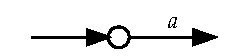
\includegraphics{parsing/basecase1}
  \caption{Fragment accepting a single character \textit{a}}
  \label{fig:basecase1}
\end{figure}

The second base fragment corresponds to the empty regular
expression. The NFA fragment is shown in figure
\vref{fig:basecase4}. One state with a single edge marked as a
$\upvarepsilon$-edge is added. The new state is the initial state for
this fragment and the edge is left dangling. This fragment is used for
the empty regular expression and for alternations with one or more
options left empty.

%% In Ken Thompson article from 1968 \cite{Thompson1968}, in
%% \cite{HopcroftJohnE.AndMotwaniRajeevAndUllman2001} and in
%% \cite{RussCox} a method for converting a regular expression to an
%% automaton is described.



%% The base case is the regular expression consisting of a single
%% character \textit{a}. Figure \vref{fig:basecase1} shows an automaton
%% accepting the same language. 

\begin{figure}
  \centering
  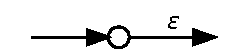
\includegraphics{parsing/basecase4}
  \caption{Fragment accepting the empty string}
  \label{fig:basecase4}
\end{figure}


%% \begin{figure}
%%   \centering
%%   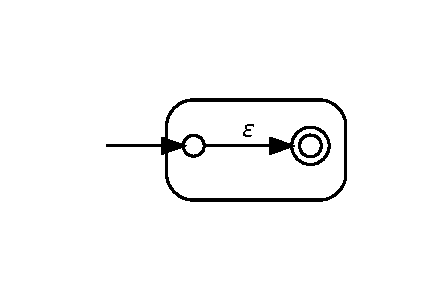
\includegraphics{parsing/basecase3}
%%   \caption{The empty string}
%%   \label{fig:basecase3}
%% \end{figure}

The first compound fragment is alternation, see figure
\vref{fig:alternation}. Here, the two sub-fragments R and S are automatons
with initial states and some dangling edges. What else they are
composed of, is irrelevant for the moment\todo{changed}. We add one new state, 
and make it the initial state for this fragment. The initial state has two
$\upvarepsilon$-edges leaving, connecting to the initial states of R
and S. The dangling edges for the new fragment is the sum of the
dangling edges leaving R and S.

\begin{figure}
  \centering
  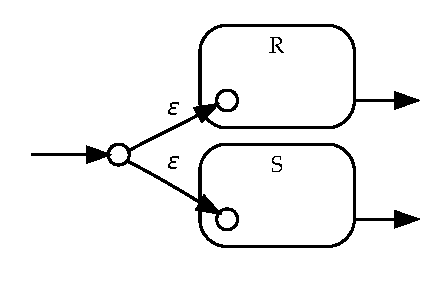
\includegraphics{parsing/alternation}
  \caption{Alternation R\textbar S}
  \label{fig:alternation}
\end{figure}

Concatenation of two regular expressions R and S is achieved as shown
in figure \vref{fig:concatenation}. The dangling edges of R is
connected to the initial state of S. The initial state for the new
fragment is the initial state of R and the dangling edges of S is
still left dangling.

\begin{figure}
  \centering
  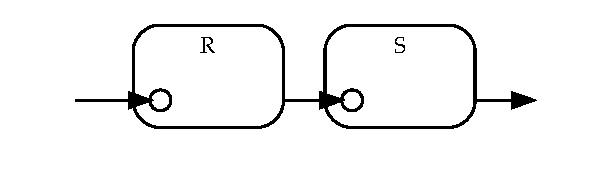
\includegraphics{parsing/concatenation}
  \caption{Concatenation RS}
  \label{fig:concatenation}
\end{figure}

Zero or more times repetition is shown in figure
\vref{fig:repetition}. One new, initial, state is added. It has two
$\upvarepsilon$-edges leaving, one is connected to the initial state of
R and one is left dangling. The dangling edges of R is connected to
the new initial state.

\begin{figure}
  \centering
  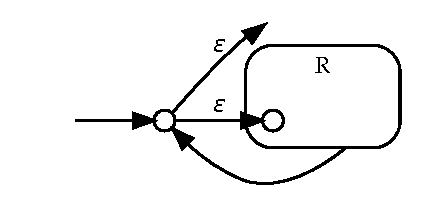
\includegraphics{parsing/repetition}
  \caption{Repetition R*}
  \label{fig:repetition}
\end{figure}

Finally an accepting state is patched into the NFA. All edges left
dangling is connected to the accepting state. 

\paragraph{Properties} NFAs created with Thompsons method has these
properties:
\begin{itemize}
  \item At most two edges is leaving a state
  \item There are no edges leaving the accepting state
  \item There are no edges leading into the starting state
\end{itemize}


\begin{example}[Converting a regular expression to a NFA]
\label{ex:converting_a_regular_expression_to_a_nfa}
\begin{figure}
  \centering 
  \subfigure[Fragment for \textsf{a}]{
    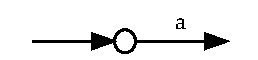
\includegraphics{parsing/ex_a.pdf}
    \label{fig:ex_parsing_a}
  }
  \subfigure[Fragment for \textsf{b}]{
    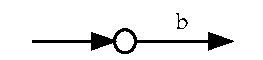
\includegraphics{parsing/ex_b.pdf}
    \label{fig:ex_parsing_b}
  }
  \subfigure[Fragment for \textsf{c}]{
    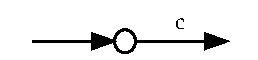
\includegraphics{parsing/ex_c.pdf}
    \label{fig:ex_parsing_c}
  }
  \subfigure[Fragment for \textsf{a*}]{
    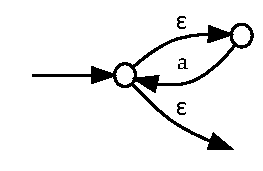
\includegraphics{parsing/ex_star.pdf}
    \label{fig:ex_parsing_star}
  }
  \subfigure[Fragment for \textsf{a*b}]{
    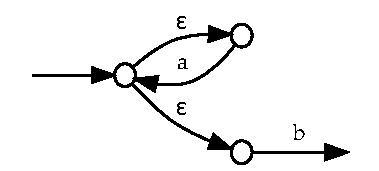
\includegraphics{parsing/ex_concat.pdf}
    \label{fig:ex_parsing_concat}
  }
  \subfigure[Fragment for \textsf{a*b\textbar c}]{
    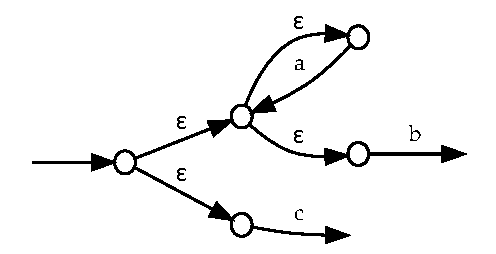
\includegraphics{parsing/ex_alt.pdf}
    \label{fig:ex_parsing_alt}
  }
  \subfigure[Final NFA for \textsf{a*b\textbar c}]{
  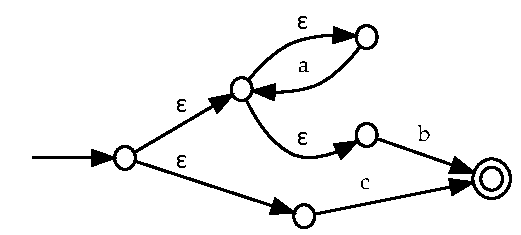
\includegraphics{parsing/ex_finished.pdf}
  \label{fig:ex_parsing_finished}
  }
  \caption{Individual fragments when converting \textsf{a*b\textbar c}
    to NFA}
  \label{fig:ex_parsing}
\end{figure}

\begin{figure}
\end{figure}


In this example we will be converting the regular expression
\textsf{a*b\textbar c} to a NFA using Thompsons method.
\begin{itemize}
\item Top level we have the alternation operator, but before we can
  complete this fragment, we need to convert \textsf{a*b} and
  \textsf{c} to fragments.
  \begin{itemize}
  \item \textsf{a*b} is complicated since we have one operator, two
    literals and a hidden concatenation. Top level we have the
    concatenation operator, concatenating \textsf{a*} and
    \textsf{b}. These needs to be converted before we can concatenate.
    \begin{itemize}
    \item \textsf{a*} needs to be broken further down. Top level we have
      the Kleene star, but we can not apply the rule for converting this
      to a NFA fragment before we have converted \textsf{a}. 
      \begin{itemize}
        \item \textsf{a} is straightforward, we just apply the rule
          for transforming literals and we have the fragment in figure
          \ref{fig:ex_parsing_a}
      \end{itemize}
      Using this fragment to complete the Kleene star, we have the
      fragment in figure \ref{fig:ex_parsing_star}.
    \item \textsf{b} is straightforward, we just apply the rule for
      transforming literals and we have the fragment in figure
      \ref{fig:ex_parsing_b}.
    \end{itemize}
    Now we are ready to concatenate, fragments
    \ref{fig:ex_parsing_star} and \ref{fig:ex_parsing_b} are
    concatenated and we have the fragment in figure \ref{fig:ex_parsing_concat}
  \item \textsf{c} is straightforward, we just apply the rule for
    transforming literals and we have the fragment in figure
    \ref{fig:ex_parsing_c}.
  \end{itemize}
  With these expressions converted to fragments we can apply the
  alternation conversion rule. We have the resulting fragment in
  figure \ref{fig:ex_parsing_alt}
\end{itemize}

All that is left now is to connect the dangling edges to an accepting
state. We have the final result in figure \vref{fig:ex_parsing_finished}
  
\end{example}

\subsection{Matching}

The NFAs constructed as described in section
\vref{sec:from_regular_expression_to_nfa} can be used to match a
regular expression with a string, i.e. to determine if a string belongs
to the language of the regular expression. 

Once the NFA is generated, simulating it is a straightforward
task. Again, our method is attributed to Thompson
\cite{Thompson1968}. 
\begin{enumerate}
    \item We maintain a set of active states and a pointer
    to the current character in the string
    \item At the beginning only the
    start state belongs to the set of active states
    \item The string is read
    from left to right, taking each character in turn. When a character is
    read from the input string, all legal transitions from the states in
    the active set is followed
    \item A transition is legal if it is a
    $\upvarepsilon$-transition or if the mark on the transition matches
    the character read from the input string. The new set of active states
    is the set of end states for the transitions followed
    \item If the
    accepting state is included in the active set when the string is read,
    the string matches the regular expression
\end{enumerate}

With this method we only ever add a state to the active set once per
iteration and we only read each character from the input string once.


\begin{example}[Matching with a NFA]
  \begin{figure}
    \centering
    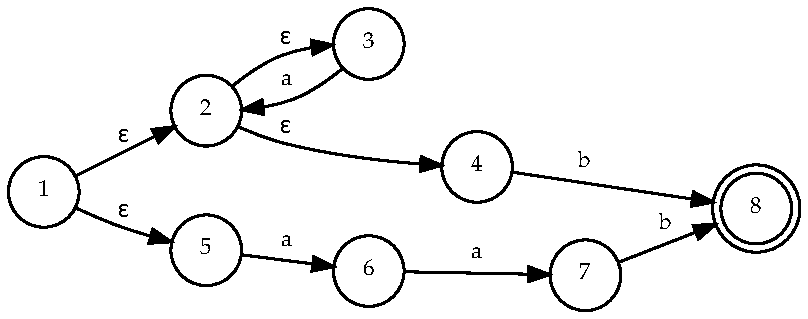
\includegraphics[width=\textwidth]{matching/ex_matching.pdf}
    \caption{NFA for the regular expression \textsf{a*b\textbar aab}}
    \label{fig:ex_matching}
  \end{figure}
  
  In this example we will demonstrate how the regular expression
  \textsf{a*b\textbar aab} is matched with the string \textsl{aab}. In
  figure \vref{fig:ex_matching} we have the corresponding NFA. Each
  state is marked with a unique number which we will be referring to
  in the table below.

\begin{center}
\begin{tabular}{ccp{8.5cm}}
Active set & \texttt{SP} & Explanation \\
\hline

1 & \textsl{\underline{a}ab} & Initially we have the start state in
the active set and \texttt{SP} points to the start of the string. \\

3, 4, 5 & \textsl{\underline{a}ab} & Following all
$\upvarepsilon$-transitions. \\

2, 6 & \textsl{a\underline{a}b} & Reading the first \textsl{a} from the input
string, states 3 and 5 have legal transitions on \textsl{a}. \\

3, 4, 6 & \textsl{a\underline{a}b} & Following all
$\upvarepsilon$-transitions. \\

2, 7 & \textsl{aa\underline{b}} & Reading the second \textsl{a} from
the input string, states 3 and 6 have legal transitions on
\textsl{a}. \\

3, 4, 6 & \textsl{aa\underline{b}} & Following all
$\upvarepsilon$-transitions. \\

8 & \textsl{aab\underline{ }} & Reading the last character from input
string: \textsl{b}, states 4 and 7 have legal transitions on
\textsl{b}. \\

8 & \textsl{aab\underline{ }} & No $\upvarepsilon$-transitions to follow.

\end{tabular}
\end{center}

After reading the string we can see that the accepting state is in the
active set: We have a match!

\end{example}



\subsection{Summary}

Regular expressions are a widely used and popular tool. The features
offered and the semantics vary. For example some will offer back
referencing and others will not, some will offer a leftmost match in
alternations, others will offer a longest match. Even for engines with
similar feature sets, the underlying implementation and performance
can vary widely. A regular expression engine can typically solve some
types of problems more efficiently than others, or vice versa: it may
be particularly bad at a given problem. %\todo{Jan: changed}

There are many highly specialized regular expression engines
exemplifying this. To briefly mention an example: Structured text like
SGML documents benefits from a different approach. Many times you will
need to find the text between two tags, but many tools are not geared
for this kind of search: The search can span several lines and we will
usually want a shortest match. See \cite{pedersen2010} for details.

To the knowledge of the writers, there is no others pursuing a regular
expression engine build on the design described in this thesis. The
division of the workload in several different components using parse
trees to communicate progress is unique. What we hope by this approach
is flexibility and a guaranteed upper bound on memory consumed for a
match.

%\todo[inline]{Might want to give an example}

%% \todo[inline]{write something about how regular expressions can be
%%   very powerful but the underlying design and its performance can vary
%% widely}

\clearpage
\section{Designing a memory efficient regular expression engine}
\label{sec:design}
\todo[inline]{Missing introduction}



\subsection{Architecture}

In this thesis we will build a general framework for matching regular
expressions with strings. Our vision is a flexible architecture where
the user is in control. Regular expression matching is a sequence of
operations, where not all operations are needed at all times. This
leads to the idea that we can split the regular expression engine into
several dedicated parts. This can be demonstrated by considering the
tasks of simple acceptance and extractions of groupings, the first
only reports if a string matches a regular expression and the latter
will also report on any groupings. By pulling this functionality out
of the regular expression engine, we make the job of reporting simple
acceptance simpler.

Before moving on, there are some prerequisites that must be
discussed. This leads us to a discussion on possible mechanisms that
would allow us to separate each task. We require several things: a
mechanism to construct a NFA, a means of generate a syntax tree and a
compact means of passing on the current state of the match process.


\subsubsection{Constructing an NFA}
In this thesis we have chosen to use Thompsons method of constructing
NFAs. The NFAs constructed in this manner exhibit desirable
properties: All states has no more than two outgoing transitions and
the number of states grows linear in the size of the regular
expression. Typically you would take this one step further and in some
way build a DFA from the NFA, since these has much better traversal
properties. We will not be doing this; the worst-case behavior of
building a DFA is exponential both in time and space, as we will see
in the evaluation section, and a DFA does not hold any particular useful 
properties for us over an NFA\todo{Jan: I think. Why?}.

\subsubsection{Dubè and Feeley}
One way of communicating the current state of the match process, would
be to send the whole parse tree. An efficient algorithm for parsing
with regular expressions is presented by Dubè and Feeley in their
paper from 2000 \cite{Dube2000}. The algorithm produces a parse tree,
describing how string $w$ matches regular expression $r$. For a fixed
regular expression the algorithm runs in time linear in the size of
$w$.

To build the parse tree, we first construct a NFA corresponding to
$r$. The article specifies a method for construction, but this can be
any NFA constructed so that the number of states is linear in the
length of $r$, this includes those constructed with Thompsons method\cite{Thompson1968}. This restriction ensures the runtime
complexity. Until this point there is no difference from a standard
NFA, but Dubé and Feeley then add strings to some of the edges. These
strings are outputted whenever the associated edge is followed. When
the outputted strings are then read in order they form a parse tree.

The idea of having output attached to edges is further developed in
the paper \cite{Henglein2010}. The parse trees Dubè and Feeleys method
yields are rather verbose and can be more compactly represented:
Whenever a node has more than one leaving edge, a string is added to
the each leaving edge\todo{jan: changed}, containing just enough information to decide which
edge was taken.


\subsubsection{Bit-values and mixed bit-values}

Henglein and Nielsen introduce the notion of bit-values in
\cite{Henglein2010}. A bit-value is a compact representation of how a
string matches a regular expression. In itself it is just a sequence of
\texttt{0}s and \texttt{1}s and has no meaning without the associated
regular expression. The actual bit-value for a string is not unique
and will depend on the choice of regular expression. If the regular
expression is ambiguous and matches the string in more than one way,
there will also be more than one sequence, or bit-value, for this combination of string and regular
expression. 

However, if we rely on the property of a Thompsons NFA, that no state has more than two outgoing transitions,\todo{jan:changed} we have
a perfect mapping for the bit-values. Instead of mapping syntax tree
constructors to bit-values, we will map the outgoing transitions in
split-states to bit-values. Each time we are faced with a choice when
traversing the NFA, we will record that choice with a bit-value. This
will enable us to recreate the exact path through the NFA. See also
\cite{Dube2000}.

For reasons we will discuss later we will introduce the notion of
mixed bit-values in this thesis. When simulating the NFA we will
simultaneously be creating many bit-values which may or may not end up
in an actual match. These individual bit-values will be referred to as a
channel. Mixed bit-values is the set of all these channels\todo{jan: changed} and they are simply a
way of talking about multiple paths through the NFA.

\subsubsection{After MBV}
We have now introduced the bit-values. The bit-values enables us to
split up the work in several tasks. 
\begin{itemize}
\item The first task will be to create the mixed bit-values describing
  the paths the Thompson matching algorithm takes through the NFA. The
  first task will need the regular expression to form the NFA and the
  string for the matching. Note that there is no need to store the
  whole string, the matching processes the characters in the input
  string in a streaming fashion.
\item The next and also last step in a simple acceptance match, would
  be to check the mixed bit-values for a match. Simply scan the
  bit-values for acceptance. 
\item In extracting the values of groupings, we would need more
  tasks. We could form a task that cuts away unneeded parts of the
  parse tree. Only the parts concerned with contents of the groupings
  would be needed to actually extract the values. To do this we would
  require the regular expression to form an NFA annotated so that we
  could recognize the relevant parts of the syntax tree.
\item We have a stream of mixed bit-values. It would be necessary at
  some point to extract the channel that makes up the actual match, if
  there is one. This can not be done in a streaming fashion. When
  first encountering a new channel, we need to know whether or not it
  has a match. The only way to know this is to read the whole stream
  of mixed bit-values. This task would only need the stream of mixed
  bit-values, it has no need for the regular expression.
\item The last step in extracting the values of the groupings would be
  to output the actual values in some format. To do this we would
  require the bit-values from the match and the regular
  expression. The regular expression is so that we can form an NFA
  annotated with the positions of the groupings. 
\end{itemize}


\subsubsection{Solutions}

There are two main methods of realizing this design. We can make the
tasks be small separate programs that communicate through pipes or we
can make one program where the tasks will be processes that
communicate through some inter-process communication model. The
separate programs model has the advantage of being simpler, in that
the communication framework is already in place, we would not have to
worry about synchronization and such. The processes model would
probably have the advantage of being much faster in communicating and
a generally lower overhead, all according to which model for
inter-process communication was chosen. We have chosen the separate
programs model, because of the ease with which you can combine the
separate programs and the much simpler communication model. This also
opens up for the possibility to store the output from one task for
later use, or perhaps even piping the output to a completely different
system with for example \texttt{netcat}. \todo{jan: naevner du mulighederne nogle steder?}

The tasks will in some sense be projections performed on the mixed
bit-values and the bit-values. The programs will therefore be called
filters. 


%% \todo[inline]{What is a filter? The whole deal with the pipes!}
%% \todo[inline]{Pros and cons to filters vs other solutions}

We present the overall architecture in figure
\vref{fig:architecture}. In the first program we have the matcher,
this program will take the regular expression as an argument and have
the string piped in and will output the mixed bit-values that
comprises the match. The second program will take the mixed bit-values
from the first and filter out those mixed bit-values relevant to the
capturing groupings only. The third program takes mixed bit-values and
filters out the bit-values relevant to the actual match, if there is
no match, the output will be the empty string. The fourth program
takes bit-values and constructs the string that was matched with those
bit-values. If you rewrite the regular expression so that it only
consists of the capturing groups and adjust your bit-values
accordingly, this will result in the capturing groups being
outputted. We have put in a fifth, hypothetical, program in the design to signal that
you could have more filters and place them anywhere in the chain (though there are some common sense limitations)
\begin{figure}
  \centering
  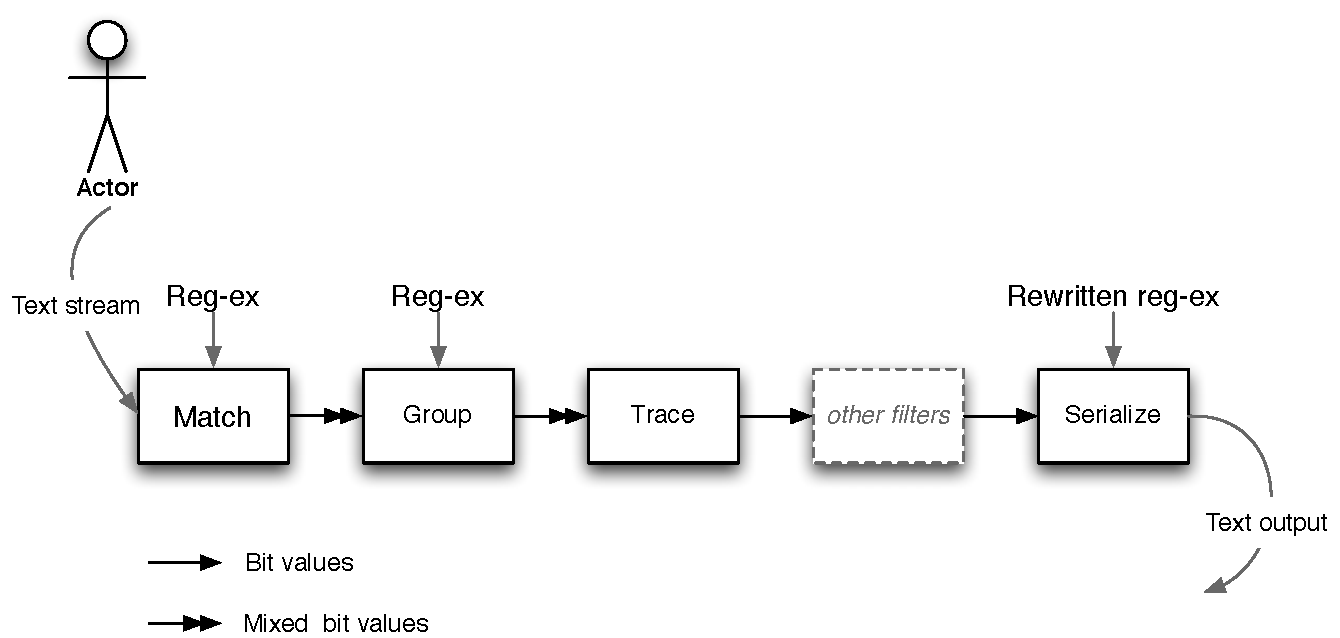
\includegraphics[width=\textwidth]{design/architecture.pdf}
  \caption{Architecture outline}
  \label{fig:architecture}
\end{figure}


%% \todo[inline]{
%% Fleksibel arkitektur (skal tales om sent, det er en implementeringsting):
%%  - hvorfor som unix utility. Plus: nemt at søtte sammen on the fly,
%%  kan nemt serialisiere og transmittere output
%%  - andre alternativer: in-process components. Hvad er drawback: fx
%%  mere bøvlet at sætte sammen on the fly. Hvad er plus: hurtigere
%%  kommunikation mellem komponenter. Reuse af NFA.
 
%% Mixed-bit-values:
%%  Motivation: ?? (kompression?)
%%  Valgmuligheder: alternativer (IKKE IMPLEMENTATION)
%%  Valg
%% }

\subsection{Protocol specification}
\label{sec:protocol_spec}

%\todo[inline]{Introduce the mixed bit-values term.}

In this section we will define a protocol that can communicate
information between our programs. The information consists of the
mixed bit-values generated by the NFA simulator and the filters. The
protocol should enable us to recreate paths taken through an NFA. 

This protocol is intended to communicate at a machine level between programs where we can expect perfect synchronization and unambiguity. For this reasons, our protocol is very compact. The actual implementation may use different symbols to represent the operators below.\todo{jan: added}

We need our protocol to support the following operators. A description is supplied for each.

\begin{description}
  \item[\textbar] The end of the channel list is reached and we should
    set the active channel to the first channel. This coincides with
    reading a new character. It is not a strictly necessary operator,
    we can make do with the change channels action. We choose to keep
    a separate action for end of list, because it adds to readability
    and redundancy.
  \item[:] Whenever we change channels we put a :. There may be more
    than one or perhaps even no bits output on a channel for any given
    character from the string
  \item[=] Copying of a channel. One channel is split into two, the
    paths taken through the NFA will be identical up to the point of
    splitting. The newly created channel is put in front of the rest
    of the channels
  \item[0,1, \textbackslash $a$] The actual bit values. The character
    classes needs extra care as we need to know on\todo{jan: what?} which character we
    passed them, so we put the value we pass on, escaped in the output
  \item[b] A channel is abandoned with no match
  \item[t] A channel has a match
\end{description}

\begin{example}[Protocol]
  In figure \vref{fig:ex_prot} we have an automaton for regular
  expression \textsf{a*}. When matching this regular expression with
  the string \textsl{aa} we generate some mixed bit-values. This
  example will in detail demonstrate how the mixed bit-values are
  generated.
  \begin{figure}
    \centering
    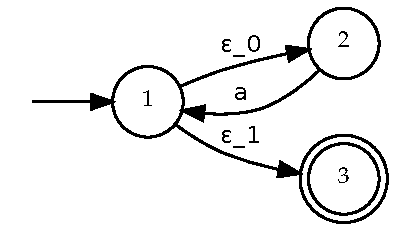
\includegraphics{matching/example_protocol.pdf}
    \caption{Automaton with bitvalues for regular expression
      \texttt{a*}}
    \label{fig:ex_prot}
  \end{figure}
  
  \begin{description}
  
  \item[Initial step:] Initially the start state of the automaton is
    added to the active list. All $\upvarepsilon$-edges are followed
    and the following is output:
    \begin{enumerate}
    \item Node 1 is a split-node, a \texttt{=} is output, and we
      follow the $\upvarepsilon$-edge to node 2 and output a
      \texttt{0}. We can not make any further progress on this
      channel. We output a \texttt{:} and switch to the next channel.

      Output so far: \texttt{=0:}. \\
      List of active channels: $\{2, 1\}$.
    \item The active channel is now in node 1, we follow the
      $\upvarepsilon$-edge from node 1 to 3 and output a
      \texttt{1}. We can not make any further progress on this
      channel. This is the last channel in the channel list, so we
      output a \texttt{|} and reset the active channel.

      Output so far: \texttt{=0:1|}.\\
      List of active channels: $\{2, 3\}$.
    \end{enumerate}

  \item[First \textsl{a} is read]
    \begin{enumerate}
    \item Node 2 has a transition marked \texttt{a}, we follow this
      back to node 1. Node 1 is a split-node, a \texttt{=} is output,
      and we follow the $\upvarepsilon$-edge to node 2 and output a
      \texttt{0}. We can not make any further progress on this
      channel. We output a \texttt{:} and switch to the next channel.

      Output so far: \texttt{=0:1|=0:}. \\
      List of active channels: $\{2, 1, 3\}$.
    \item The active channel is now in node 1, we follow the
      $\upvarepsilon$-edge from node 1 to 3 and output a
      \texttt{1}. We can not make any further progress on this
      channel. We output a \texttt{:} and switch to the next channel.

      Output so far: \texttt{=0:1|=0:1:}. \\
      List of active channels: $\{2, 3, 3\}$.
    \item Node 3 is the accepting node and does not have any
      transitions. We abandon this channel and output a
      \texttt{b}. This is the last channel in the channel list, so we
      output a \texttt{|} and reset the active channel.

      Output so far: \texttt{=0:1|=0:1:b|}. \\
      List of active channels: $\{2, 3\}$.
    \end{enumerate}
  \item[Second \textsl{a} is read] This is the final step.
    \begin{enumerate}
      \item From node 2 we can make a transition on \texttt{a} back to
        node 1. This is a split node, so we output a \texttt{=} and
        transition on the the $\upvarepsilon$-edge to node 2 and
        output a \texttt{0}. We can not do further transitions and
        this is not the accepting node, we abandon this channel and
        output a \texttt{b}. We switch to the next channel and output
        a \texttt{:}.

        Output so far: \texttt{=0:1|=0:1:b|=0b:}. \\
        List of active channels: $\{1, 3\}$.
      \item Node 1 has a $\upvarepsilon$-transition to node 3, we take
        it and output a \texttt{1}. We can not do further transitions
        and since this is the accepting node, we output a
        \texttt{t}. We have one channel left, so we output a
        \texttt{:} and switch.

        Output so far: \texttt{=0:1|=0:1:b|=0b:1t:}. \\
        List of active channels: $\{3\}$.
      \item Node 3 has no available transitions. We abandon this
        channel and output a \texttt{b}.

        Output so far: \texttt{=0:1|=0:1:b|=0b:1t:b}. \\
        List of active channels: $\{\}$.
    \end{enumerate}
  \end{description}
\end{example}

\subsection{Filters}

We have now established that filters are stand-alone programs that
takes input, performs some projection and outputs the result. In this
subsection we will give a more detailed description of the filters
developed for this thesis. 

The filters can be combined to make a whole, naturally some orders of
combining makes more sense than others. For example will it make sense
to have filters removing unnecessary information as early as possible,
to reduce the input data-sizes for downstream filters.

%% \todo[inline]{Better introduction or consider merging with architecture}

%% \todo[inline]{Describe orders of filters}


\subsubsection{The 'match' filter}

\paragraph{Input} Any mixed bit-values or bit-values
\paragraph{Output} A single value indicating match or no match.
\paragraph{}

This is a simple filter. The input is scanned for a \texttt{t} control
character, if present we output a \texttt{t} otherwise we output a
\texttt{b}. In the case of empty input, we will output an error
message, this is because the empty input is most likely due to an
error in the previous programs. To save time on processing, we will
assume the input format is correct.

\begin{example}
The regular expression \textsf{a*} matches the string \textsl{aaa}:
\begin{verbatim}
$ echo -n 'aaa' | ./main 'a*' | ./ismatch 
t
\end{verbatim}
\textsf{a*} does \emph{not} match \textsl{bbb}:
\begin{verbatim}
$ echo -n 'bbb' | ./main  'a*' | ./ismatch 
b
\end{verbatim}
Since we do not check the correctness of the input, the sentence:
``the cake is a lie'' which is clearly not in the correct input format
with regards to the protocol defined section \vref{sec:protocol_spec},
will also produce a positive answer from the filter:
\begin{verbatim}
$ echo -n 'the cake is a lie' | ./ismatch
t
\end{verbatim}

\end{example}

\subsubsection{The 'trace' filter}
\label{sec:desc_materialize}
\paragraph{Input} Mixed bit-values
\paragraph{Output} Bit-values
\paragraph{}

The mixed bit-values is a way of keeping track of multiple paths
through the NFA. This filter will remove all channels from the mixed
bit-values, except the one that has a match. We are using
Thompsons method for matching, so we can be sure there is at most one
channel with a match. 

This will be a non-streaming filter. This problem can not be solved
without in some way storing the mixed bit-values: We need knowledge of
whether or not a channel has a match at the beginning, but we will not
have that knowledge until the end.

\begin{example}
In the previous example we saw that the regular expression \textsf{a*}
matches the string \textsl{aaa}. The NFA for the regular expression is
in figure \vref{fig:ex_prot}, marked with state numbers and
bit-values. This particular match will generate the following mixed
bit-values: \texttt{=0:1|=0:1:b|=0:1:b|=0b:1t:b}. The filter should
then only return the bit-values \texttt{0001}, which represents the
match. The filter should return the empty string if there is no match.
\end{example}


\subsubsection{The 'groupings' filter}
\label{sec:groupings_filter_analysis}
\paragraph{Input} Mixed bit-values
\paragraph{Output} Mixed bit-values for rewritten regular expression
\paragraph{}

This filter facilitates reporting the content of captured groups. The
filter outputs the mixed bit-values associated with the groupings. By
this we mean that all mixed bit-values generated while inside a
captured group should be sent to output and all mixed bit-values
generated outside a group should be thrown away. By throwing away the
unnecessary bit-values we hope to make the mixed bit-values sequence
shorter. This will be an advantage when the time comes to apply the
trace filter, which is non-streaming, described in section
\vref{sec:desc_materialize}.

\begin{example}[Simple groupings filter]
  \label{ex:simple_groupings}
  Here we have a few simple examples of what the groupings filter
  should do. 
  \begin{itemize}
  \item
    For regular expression \textsf{(a\textbar b)} matched with
    \textsl{a} the mixed bit-values are \texttt{=0:1\textbar t:b}. Since
    the whole regular expression is contained in a capturing
    parenthesis, nothing should be thrown away. Output should contain
    \texttt{=0:1\textbar t:b}.
  \item
    For regular expression \textsf{(?:a\textbar b)(c\textbar d)} matched
    with \textsl{ac} the mixed bit-values are
    \texttt{=0:1|=0:1:b|t:b}. This time the first part of the regular
    expression is contained only in a non-capturing parenthesis and the
    associated bit-values should be thrown away. We want to keep only the
    bit-values from the second alternation. Output should contain
    \texttt{=:|=0:1:b|t:b}.
  \end{itemize}
  
  In this example we have only dealt with simple examples. Regular
  expressions containing parenthesis under alternation and repetition,
  e.g. \textsf{(a)\textbar b} and \textsf{(a)*}, require extra care
  and will be discussed later.
\end{example}

The output of the groupings filter can be used to navigate the NFA for
the regular expression altered in a similar manner: Everything not in
a capturing parenthesis is thrown away. From example
\vref{ex:simple_groupings} we have the regular expression
\textsf{(?:a\textbar b)(c\textbar d)}, if we throw away everything not
in a capturing parenthesis we have left \textsf{(c\textbar d)}. Stated
in a more formal manner, we can define our first naive rewriting
function $G'$:

\begin{align}
  G'[[\upvarepsilon]] &= \upvarepsilon \notag\\
  G'[[a]] &= \upvarepsilon \notag\\
  G'[[ [...] ]] &= \upvarepsilon \notag\\
  G'[[r'r_2]] &= G'[[r']]G'[[r_2]] \notag\\
  G'[[r'|r_2]] &= G'[[r']]G'[[r_2]] \notag\\
  G'[[r*]] &= G'[[r]] \notag\\
  G'[[r+]] &= G'[[r]] \notag\\
  G'[[r?]] &= G'[[r]] \notag\\
  G'[[(?:r)]] &= G'[[r]] \label{eq:G1_paren}\\
  G'[[(r)]] &= (r) \notag
\end{align}

\paragraph{Capturing under alternation}
As is seen, $G'$ basically throws away anything not in a capturing
parenthesis. There are however a few problems with this definition, as
hinted earlier. Our first problem is regular expression with a
capturing parenthesis under alternation. When the capturing
parenthesis is under the alternation and we throw away the
alternation, we lose a vital choice: There is no longer a way to
signal whether or not a group participates in a match.
\begin{figure}
  \centering
  \subfigure[\textsf{(a)\textbar (b)}]{
    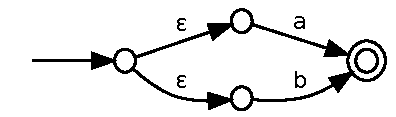
\includegraphics{filters/capturing_under_parenthesis1.pdf}
    \label{fig:capt_paren1}
  }
  \subfigure[\textsf{(a)(b)}]{
    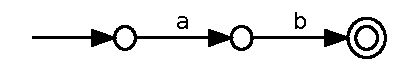
\includegraphics{filters/capturing_under_parenthesis2.pdf}
    \label{fig:capt_paren2}
  }
  \subfigure[\textsf{(?:\textbar (a))(?:\textbar (b))}]{
    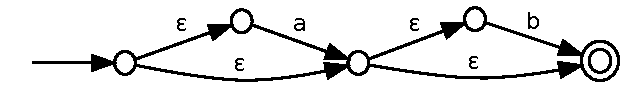
\includegraphics{filters/capturing_under_parenthesis3.pdf}
    \label{fig:capt_paren3}
  }
\caption{Capturing under alternation}
\end{figure}

\begin{example}[Capturing under alternation]
  \label{ex:capturing_under_alternation}
  In matching the regular expression \textsf{(a)\textbar (b)}, see
  figure \vref{fig:capt_paren1} for the NFA, with the string
  \textsl{a} we obtain these mixed bit-values: 
  \begin{center}\texttt{=0:1|t:b}\end{center}
  What these mixed bit-values are saying is that we have 2 channels,
  one that go through \textsf{a} and succeeds and one that go through
  \textsf{b} and fails. The succeeding channel never goes through
  \textsf{b}, the contents of that group is not defined.
  
  Rewriting the regular expression \textsf{(a)\textbar (b)} according
  to $G'$ we have:
  \begin{align*}
    G'[[\text{\textsf{(a)\textbar (b)}}]] &=
    G'[[\text{\textsf{(a)}}]]G'[[\text{\textsf{(b)}}]] \\
    &= \text{\textsf{(a)}}\text{\textsf{(b)}} \\
  \end{align*}
  In this regular expression there is only one way: The one going
  through both the groups. See figure \vref{fig:capt_paren2} for the
  NFA of the expression. This is bad news for our rewriting function
  and our filter, since we need some way of skipping groups: Each
  channel goes through only one group.
\end{example}

In example \ref{ex:capturing_under_alternation} we saw an example of
how undefined groups are not handled. To solve this problem we need
some way of signaling if a group participates in a match or not. We
define a new rewriting function $G''$ it is identical to $G'$ except
for equation \ref{eq:G1_paren} which is changed to:
\begin{align}
    G''[[(r)]] &= (?:|(r)) \notag
\end{align}
This change will enable us to choose which groups participates in a
match. This comes at a cost: Extra bits will have to be added to the
mixed bit-values output and extra alternations to the rewritten
regular expression. 

\begin{example}[continues=ex:capturing_under_alternation]
With the changed equation \ref{eq:G1_paren} we can continue our
example from before. Again we rewrite regular expression
\textsf{(a)\textbar (b)}, this time according to $G''$:
  \begin{align*}
    G''[[\text{\textsf{(a)\textbar (b)}}]] &=
    G''[[\text{\textsf{(a)}}]]G''[[\text{\textsf{(b)}}]] \\
    &= \text{\textsf{(?:\textbar (a))(?:\textbar (b))}} \\
  \end{align*}
  See figure \vref{fig:capt_paren3} for the NFA. As is clear from the
  rewritten regular expression and the NFA, there is now a way around
  the groups. Taking this into account, the output for the groupings
  filter should be: 
  \begin{center}\texttt{=1:01|0t:b}\end{center}
  What these mixed bit-values are saying is that we have two channels,
  one picks the route through \textsf{a}, around \textsf{b} and
  succeeds and the other picks the route around \textsf{a}, through
  \textsf{b} and fails.
\end{example}
As needed, we now have a way of signaling if a particular group is in
a match: Insert a 1 in the mixed bit-values and the group participates
or insert a 0 and it does not. 


\paragraph{Capturing under repetition}
The other problem we hinted at has to do with capturing under
repetition. When using a capturing subpattern, it can match repeatedly
using a quantifier. For example matching \textsf{(.)*} with the string
\textsl{abc}, the first time we apply the \textsf{*} we capture a
\textsl{a} the second time a \textsl{b} and the last time a
\textsl{c}. In such a case we have several options when reporting the
strings that was captured:
\begin{itemize}
\item The first
\item The last, this is the what most backtracking engines like Perl
  do
\item All, this is what a full regular expression engine do
\end{itemize}
Only two of these options are available to a streaming filter: All and
the first. In order to return the last match, we would have to save
the latest match when matching with the quantifier, it is potentially
the last and we can not know until we are done matching with the
quantifier.

Returning the first string that was captured by the quantifier, forces
us to throw away mixed bit-values generated in a capturing
parenthesis. We would only need the mixed bit-values generated by the
first iteration of the quantifier. 

To return all the strings captured by a group, we simply output all
the mixed bit-values generated while in the capturing
parenthesis. However, this causes problems with the rewriting
function. Rewriting \textsf{(.)*} according to $G''$ we have
\textsf{(.)}. This regular expression accepts one single character. In
no way can we make mixed bit-values, fitting this regular expression,
that represent a list of matched strings. Therefore we add the
following equations:
\begin{align*}
  G''[[(r)*]] &= (r)* \\
  G''[[(r)+]] &= (r)+
\end{align*}
We should now also keep the mixed bit-values that glues the iterations
together, even though they are outside the capturing group.




%% \begin{example}[Capturing under repetition]
%%   %% \begin{figure}
%%   %%   \centering
%%   %%   \subfigure[\textsf{(a)*}]{
%%   %%     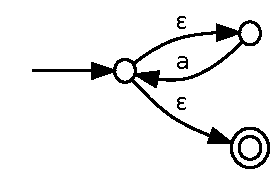
\includegraphics{filters/capt_under_rep1.pdf}
%%   %%     \label{fig:capt_rep1}
%%   %%   }
%%   %%   \subfigure[\textsf{(a)}]{
%%   %%     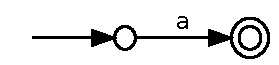
\includegraphics{filters/capt_under_rep2.pdf}
%%   %%     \label{fig:capt_rep2}
%%   %%   }
%%   %%   \caption{Capturing under repetition}
%%   %% \end{figure}

%%   %% In this example we will be matching regular expression
%%   %% \textsf{(a)*}, see figure \vref{fig:capt_rep1} for the NFA, with the
%%   %% string \textsl{aaa}. This match generates the following mixed
%%   %% bit-values:
%%   %% \begin{center}\texttt{=0:1|=0:1:b|=0:1:b|=0b:1t:b}\end{center}

%%   %% Rewriting \textsf{(a)*} according to $G''$ gives us:
%%   %% \begin{align*}
%%   %%   G''[[\text{\textsf{(a)*}}]] &= G''[[\text{\textsf{(a)}}]] \\
%%   %%   &= \text{\textsf{(a)}}
%%   %% \end{align*}
%%   %% See figure \vref{fig:capt_rep2} for the NFA.

%%   %% This rewrite works if we are only interested in one 

%%   By matching
%% \end{example}


%% To return all we need to make some changes to the rewriting function,
%% we add the following equations:
%% \begin{align*}
%%   G''[[(r)*]] &= (r)* \\
%%   G''[[(r)+]] &= (r)+
%% \end{align*}


%% We should not just throw away everything

%% If we choose to return all, all we need to do is add equations to the
%% rewriting function:
%% \begin{align*}
%%   G''[[(r)*]] &= (r)* \\
%%   G''[[(r)+]] &= (r)+
%% \end{align*}



%% Returning all would be the easier solution. We need to be careful when
%% rewriting the regular expression however. With the output from the
%% groupings filter we should be able to navigate the NFA for the
%% rewritten regular expression.


%% Returning all would be the easiest solution, this would however
%% require a change in the rewriting function. We add the equations:
%% \begin{align*}
%%   G''[[(r)*]] &= (r)* \\
%%   G''[[(r)+]] &= (r)+
%% \end{align*}


%% %% Returning all of the strings that were captured is by far the easiest,
%% %% no extra work is required. On the other hand if we only want to return
%% %% the first of the matches, we need to know whether or not to return a
%% %% particular match, that is if this is the first time we match with the
%% %% quantifier or not. If we alter the way we construct the NFA, we can
%% %% achieve this. 





%% \todo{Hvad den blippen er det nu for en løsning jeg har på det
%%   problemos}



We are now ready to present the final rewriting function: Definition
\vref{def:G}.
\begin{definition}[The groupings filter rewriting function]
  \label{def:G}
  For regular expressions $r$, $r_1$, $r_2$, defined over alphabet
  $\Sigma$, and $a$, any character from $\Sigma$, let $G$ be defined by:
  \begin{align*}
    G[[\upvarepsilon]] &= \upvarepsilon \\
    G[[a]] &= \upvarepsilon \\
    G[[ [...] ]] &= \upvarepsilon \\
    G[[r_1r_2]] &= G[[r_1]]G[[r_2]] \\
    G[[r_1|r_2]] &= G[[r_1]]G[[r_2]] \\
    G[[r*]] &= G[[r]] \\
    G[[r+]] &= G[[r]] \\
    G[[r?]] &= G[[r]] \\
    G[[(?:r)]] &= G[[r]] \\
    G[[(r)]] &= (?:|(E)) \\
    G[[(r)*]] &= (?:|(r)*) \\
    G[[(r)+]] &= (?:|(r)+) \\
  \end{align*}
\end{definition}
\begin{example}
  Here follows a few examples of how the groupings filter rewriting
  function, $G$, works.
  \begin{align*}
    G[[\mathsf{(a)|b}]] &= G[[\mathsf{(a)}]]G[[\mathsf{b}]]\\
    &= \mathsf{(?:(a))} \upvarepsilon\\
    &= \mathsf{(?:(a))}
  \end{align*}

  \begin{align*}
    G[[\mathsf{((cup)cake)}]] &= \mathsf{(?:|((cup)cake))}
  \end{align*}

  \begin{align*}
    G[[\mathsf{(a|b)*}]] &= \mathsf{(a|b)*}
  \end{align*}
\end{example}



\clearpage
\section{Implementing a regular expression engine}
\label{sec:implementation}
The task of implementing a regular expression engine can be undertaken
in steps. The first steps is converting the regular expression to a
NFA. The next step is to simulate the NFA. The last step in our
implementation is to build filters.

%% \subsection{Datastructures}

%% \subsubsection{Representing the NFA}

%% For the representation of the NFA we started out as Russ Cox in
%% \cite{RussCox}. The NFA is represented as a linked collection of
%% \lstinline{State} structures:
%% \begin{lstlisting}
%% struct State
%% {
%%     unsigned int c;
%%     unsigned int type;
%%     struct State *out0;
%%     struct State *out1;
%% };
%% \end{lstlisting}
%% This is the essential contents of the \lstinline{State} structure. It
%% actually contains more variables, these will be added and explained
%% when appropriate. There is no explicit representation of the
%% transitions, they are represented as the two \lstinline{out} pointers in
%% the \lstinline{State} structure. The \lstinline{type}-variable decides the
%% type of the state and the transition(s):
%% \begin{description}
%% \item[split] This state is a split-state, both the two
%%   \lstinline{out}-pointers will be set to valid states.
%% \item[accepting] This is the accepting state.
%% \item[literal] This state only has a valid transition on the
%%   \lstinline{out0}-pointer. It is marked with the value in \lstinline{c}
%% \item[range] This is a state with a range-transition. These will
%%   be explained later in \vref{sec:ranges_impl}.
%% \item[epsilon] The transition in \lstinline{out0} is a
%%   $\upvarepsilon$-transition.
%% \end{description}

\subsubsection{Character classes}
\label{sec:ranges_impl}

\begin{figure}
  \centering 
  \subfigure[\textsf{[a-c]}]{
    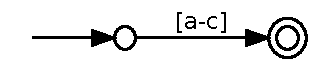
\includegraphics{implementation/range1.pdf}
    \label{fig:range1}
  }
  \subfigure[\textsf{a\textbar b\textbar c}]{
    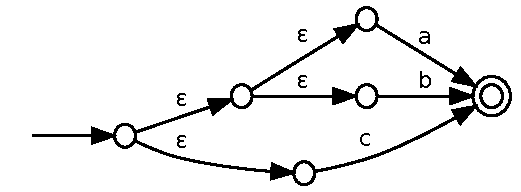
\includegraphics{implementation/range2.pdf}
    \label{fig:range2}
  }
  \caption{A simple character class-transition example}
  \label{fig:ranges}
\end{figure}

Character classes are part of the extension we made to the regular
expression definition. When implementing, we have the choice of
rewriting character classes in terms of the original regular
expressions, but as we can see in figure \vref{fig:ranges}, this
quickly becomes unwieldy. When we rewrite we add almost two states per
character matched by the character class, instead of adding just one
state for the whole character class. What we want is a NFA similar to
figure \ref{fig:range1}, not figure \ref{fig:range2}.

There are several ways of obtaining this goal. Perl uses a bitmap to
indicate membership of a range, for each character in the character
set there is a bit in the bitmap. To decide membership the bit
corresponding to the character is looked up. RE2 uses a balanced
binary tree, each node in the tree corresponds to either a whole range
or a literal character, the tree is then searched when deciding
membership. Each method has its advantages and drawbacks. The bitmap
is of constant size, so for small character classes, it will be
unnecessarily large, but the time to look up a value in the bitmap is
also constant and very fast. The balanced binary tree, has its
advantages for character classes with few ranges and literal
characters, since it will then be small in size and look up times. The
drawbacks are of course that it grows in size and look up times with
the character class.

For this project an even simpler solution was chosen: A simple linked
list of ranges. The literal characters will be represented as ranges
of length one. On other words, we will have one linked list per
character class, and the number of elements in each linked list is the
number of literals and ranges in the character class. Worst case we
will have to look through all members of a linked list to decide
membership of a character class. This is simplistic, but sufficient.

%% There should not be any serious
%% performance issues for simple character classes with few ranges and
%% literal characters.
%% \begin{lstlisting}
%% struct Range 
%% {
%%   unsigned int lo;
%%   unsigned int hi;
%%   struct Range *next;
%% };
%% \end{lstlisting}
%% The two unsigned integers are used to store the beginning and end of
%% the range, in the case of a single literal they are the same. The
%% \lstinline{next}-pointer points to the next range in the list. A
%% \lstinline{Range}-pointer and a flag to indicate whether or not the
%% character class is negated is added to the \lstinline{State} struct.

\subsection{Regular expression to NFA}

The first step in our regular expression engine is the regular
expression to NFA converter. As discussed in section
\vref{sec:re2nfa_thompson_theory}, the NFA is built from the regular
expression in steps from smaller NFA fragments. In order for this
method, used directly, to be successful, the regular expression has to
be in a form where the meta characters and the literals are presented
in the right order. Regular expressions with for example
\textsf{\textbar} can not simply be read from left to right and be
converted correctly. The problem with the alternation operator is that
it is an infix operator, so we only have the left hand side and not
the right hand side when we read the \textsf{\textbar} and can
therefore not complete the fragment.

Converting the regular expression to reverse polish notation, with an
explicit concatenation operator, or making a parse tree will solve
these problems. For this project neither is chosen. A third solution
to this problem is maintaining a stack where fragments and operators
are pushed and popped. This is the method that is implemented. We
tried determining the quality of the decision by comparing run times
with Russ Cox's example code \cite{Cox2007}. This did not go well due
to several reasons. The main reason is that the example code does not
do well on large examples\footnote{There are constants in the source
  code and a naive list append function} and large examples is needed
to do a reasonable comparison.

We followed Russ Cox' method from \cite{RussCox}, when converting the
regular expression to NFA. Russ Cox rewrites the regular expression to
reverse polish notation with an explicit concatenation operator, so
some changes will be necessary. There are tree main areas that needs
to be changed:

\begin{description}
\item[Concatenation] While constructing the NFA, NFA fragments are
  pushed onto a stack. Whenever the concatenation operator is
  encountered, the two top fragments are popped and patched together,
  see figure \vref{fig:concatenation}. We do not have the advantage of
  an explicit concatenation operator. Instead we will be trying to pop
  the top two NFA fragments and patching them together as often as
  possible. As often as possible is after a character is read, but
  before any action is taken on the character read. The exception to
  this rule is the quantifiers, which binds tighter than
  concatenation.
\item[Parentheses] The binding of the operators can be changed with
  parentheses. Not using a tree structure or reverse polish notation
  with an explicit concatenation operator, there is nothing showing
  the structure of how everything binds when simply reading the
  regular expression from left to right. We need some way of
  connecting the left parentheses to the matching right
  parentheses. For this we will be using the stack, we will expand it
  to also accept operators. Every time we read a left parenthesis in
  the regular expression, a left-parenthesis-fragment is pushed onto
  the stack. When we later on read a right parenthesis we simply pop
  fragments of the stack and patch them together till we reach a
  left-parenthesis-fragment.   
\item[Alternation] When reading the regular expression left to right,
  we only have the left NFA fragment ready when reading the
  alternation operator. Therefore we simply push the alternation
  operator on the stack. Whenever possible we pop the alternation
  operator and associated NFA fragments and patch them together, see
  figure \vref{fig:alternation}. This is probably not very often, as
  it will only happen after reading a right parenthesis or the end of
  the regular expression.
\end{description}


%% While constructing the NFA
%% we maintain a stack of NFA fragments. Each fragment consists of a
%% \lstinline{start} state and a list of its outgoing or dangling arrows:
%% \begin{lstlisting}
%% struct Fragment 
%% {
%%   unsigned int op;
%%   struct State *start;
%%   struct Statelist *out;
%% };
%% \end{lstlisting}
%% Here we see the first change: The \lstinline{op}-variable. This is
%% used when pushing operators on the stack. The two operators we need to
%% push is alternation and left parenthesis, so the possible values of
%% the \lstinline{op}-variable are:
%% \begin{description}
%% \item[none] This is a \lstinline{Fragment} representing a partial
%%   NFA. All \lstinline{Fragment}s with a value different from none, are
%%   not representing partial NFAs, they are merely markers.
%% \item[alternate] This \lstinline{Fragment} is a alternate marker.
%% \item[left parenthesis] This \lstinline{Fragment} is a left
%%   non-capturing left parenthesis marker.
%% \item[left capturing parenthesis] This \lstinline{Fragment} is a left
%%   capturing parenthesis marker.
%% \end{description}
%% In \cite{RussCox} Russ Cox does not need to push operators on the
%% stack, because they appear in the regular expression in the right
%% order. We need to somehow remember we have seen alternate and left
%% parenthesis operators, and the way we do this is to push them on the
%% stack. 

We have two important helper functions: \lstinline{maybe_concat} and
\lstinline{maybe_alternate}. The first concatenates the top two
fragments if possible, also see figure \vref{fig:concatenation}. The
second alternates the top fragments, if possible, so also figure
\vref{fig:alternation}. \lstinline{maybe_alternate} will pop alternate
markers from the stack. These are called as often as possible to keep
the stackdepth at a minimum and to avoid postponing all the
concatenating and alternating till the end. Supplying a regular
expression consisting entirely of left parenthesis will still make the
stackdepth grow to a maximum.

%% Whenever we encounter a right parenthesis we pop fragments of the
%% stack till we reach the left parenthesis marker fragment. The amount
%% of fragments we need to pop should not exceed one fragment after a
%% call to the helper functions \lstinline{maybe_concat} and
%% \lstinline{maybe_alternate}. If the parenthesis is empty we put in a
%% $\upvarepsilon$-transition. This is done because empty parenthesis is
%% often used instead of the empty string, which is very hard to write
%% explicitly seeing as it is empty.

\subsection{The simulator}

We have built the NFA and the next step is to simulate it. This
requires keeping track of a set of active states. In a basic
implementation of the Thompson simulation algorithm
\cite{Thompson1968}, a state is only added to the active set
once. This will throw away matches, e.g. when the regular expression
\textsf{a\textbar a} is matched with the string \textsl{a} there are
two possible routes through the NFA, but only one will be reported,
since the final state will only be added once to the set of active
states.

We had to adjust the basic implementation to our needs; we need to
generate mixed bit-values. 


We have implemented the standard Thompson simulation algorithm, but it
is possibly to report all matches, you just need to allow a state to
be added more than once to the active set. This will give rise to
infinite loops when matching regular expressions like \textsf{()*},
see figure \vref{fig:inf_loop_simple} for the NFA. The simulator will
go into a infinite loop generating these bit-values:
\begin{verbatim}
  =0=0=0=0=0=0=0=0=0=0=0=0=0=0=0=0=0=0=0...
\end{verbatim}
This is because there is a cycle of $\upvarepsilon$-transitions in the
NFA. \todo{cut out all this DFS stuff?} This would not be desirable
behavior and we would need to stop the simulation before it goes into
an infinite loop.

\begin{figure}
  \centering \subfigure[\textsf{()*}]{
    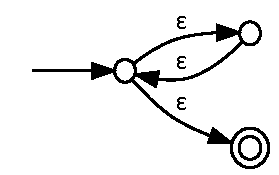
\includegraphics{implementation/inf_loop_simple.pdf}
    \label{fig:inf_loop_simple}
  }
  \subfigure[\textsf{(()())*}]{
    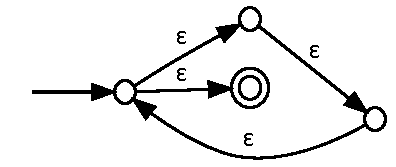
\includegraphics{implementation/inf_loop_long.pdf}
    \label{fig:inf_loop_long}
  }
  \subfigure[\textsf{(\textbar )*}]{
    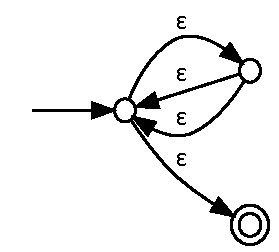
\includegraphics{implementation/inf_loop_many.pdf}
    \label{fig:inf_loop_many}
  }
\caption{$\upvarepsilon$-cycles}
\label{fig:inf_loop}
\end{figure}


From \cite{Cormen} we have the depth-first search (DFS)
algorithm. This algorithm can be modified to detect cycles. In short
it works by initially marking all vertexes white. When a vertex is
encountered it is marked gray and when all its descendants are
visited, it is marked black. If a gray vertex is encountered, then we
have a cycle and do not need to explore further on this path. The
algorithm terminates when all vertexes are black. The algorithm will
terminate, as we color one vertex each step and we always color the
vertexes darker.

To see why this algorithm detects cycles, suppose we have a cycle
containing vertex $a$. Then $a$ is reachable from at least one if its
descendants. When we reach $a$ from this descendant, it will still be
colored gray, since we are not done exploring $a$'s descendants. Thus
the cycle is detected.

Our problem is slightly different: We need to detect if we are in a
cycle of $\upvarepsilon$-transitions. The DFS algorithm solution is
still applicable, with slight modifications, as we do a depth first
search when we explore the $\upvarepsilon$-edges. There will be no
white states. Instead we will have a counter that is incremented every
time a character is read from the input string. Every time a state is
encountered it is stamped with the counter. We can only trust the
color of the state if the counter and the stamp are identical. The
gray and the black states work in much the same way.

In figure \vref{fig:inf_loop} we have some of the NFAs we
encounter. We have an example of a long cycle in figure
\ref{fig:inf_loop_long}, more parenthesis adds more
$\upvarepsilon$-transitions. We also have an example of how more
channels can be created in the loop in figure \ref{fig:inf_loop_many}
by adding alternations. 


\subsection{Filters}

\subsubsection{Groupings}

As we described in section \vref{sec:groupings_filter_analysis}, this
is the filter that should (more or less) throw away any mixed
bit-values not generated in a capturing parenthesis. In order to do
this we need to know which values are generated in a capturing
parenthesis and which are not. We look to Laurikari
\cite{laurikari2001} for inspiration. We will be using a NFA augmented
with extra $\upvarepsilon$-transitions. The extra transitions will be
used to mark the beginning and end of a capturing parenthesis. We will
use the mixed bit-values to navigate the NFA, whenever we are inside a
capturing parenthesis we will copy the mixed bit-values to output. 
\todo[inline]{Add example of the extra epsilon-edges}

We rewrote the regular expression to allow for capturing under
alternation. We will need to insert a \texttt{1} when a group
participates and a \texttt{0} when it doesn't. When exiting the upper
arm of an alternation we need to know how many top level capturing
groups there are in the lower arm and when entering the lower arm we
need to know how many top level capturing groups there in the upper
arm. Again we solve this problem by augmenting the NFA. We insert the
extra information in the split-state marking the entrance to an
alternation and add an extra state at the end of the upper arm.

\todo[inline]{Add example of the extra node and information}

We adopt a similar strategy to solve the problem of reporting only the
first match in capturing under a quantifier. We will again augment the
NFA with necessary information. A state is inserted at the end of the
quantifier, so that this state is the last state that is met in a
iteration of the quantifier. When we pass this state and do another
iteration we will know that we have already been there at least once
and should not output any more bit-values.

\todo[inline]{Add example of star iteration count thingy}


We could also have solved the problem of keeping track of how many
times we have matched a quantifier by simply rewriting the regular
expression. For example would we rewrite \textsf{(a)*} to
\textsf{(\textbar a)a*}. This was dropped because it can not be done
easily on the fly by the NFA generator. The fragment formed by
\textsf{(a)} could no longer be considered a finished fragment that
was just plugged into the rest. We use it with and without the
capturing parenthesis in the rewrite and would therefore need to open
up the fragment and remove the capturing parenthesis for parts of the
rewrite.

%% \paragraph{Capturing under repetition} When using a capturing
%% subpattern, it can match repeatedly using a quantifier. For example
%% matching \textsf{(.)*} with the string \textsl{abc}, the first time we
%% apply the \textsf{*} we capture a \textsl{a} the second time a
%% \textsl{b} and the last time a \textsl{c}. In such a case we have
%% several options when reporting the strings that was captured:
%% \begin{itemize}
%% \item The first
%% \item The last, this is the what most backtracking engines like Perl
%%   do
%% \item All
%% \end{itemize}
%% Only two of these options are available to a streaming filter: All and
%% the first. In order to return the last match, we would have to save
%% the latest match when matching with the quantifier, it is potentially
%% the last and we can not know until we are done matching with the
%% quantifier.

%% Returning all of the strings that were captured is by far the easiest,
%% no extra work is required. On the other hand if we only want to return
%% the first of the matches, we need to know whether or not to return a
%% particular match, that is if this is the first time we match with the
%% quantifier or not. If we alter the way we construct the NFA, we can
%% achieve this. 


%% \paragraph{Capturing under alternation}
%% We are also faced with a choice when values are alternated in a
%% capturing subpattern.


\subsubsection{Trace}

We will limit this filter to only output one channel with a match. In
the current system this is not actually a limitation, as we are using
Thompsons method for matching, there will only ever be one channel
with a match.

All channels are read and the bit-values are saved separately. Every
time we read a channel-split operator we will have to allocate a new
chunk of memory and copy the bit-values we have accumulated up to this
point. When the chunk of memory becomes to small, we will enlarge to a
chunk twice the size. When we reach the end of the input stream, we
will know if there is a match and be able to output the bit-values
that make up the match.


\subsubsection{Serialize}
  
This is the filter that outputs what is matched. We will need the
regular expression, that matches the bit-values, to form the NFA. The
NFA is traversed using the bit-values. As we go along we output the
symbols the transitions are marked with and the escaped symbols in the
bit-values. This should result in a string being outputted of what was
matched.

\clearpage
\section{Optimizations}
The program as described in section \vref{sec:implementation} is
unoptimized and written for readability and simplicity. This section
deals with potential and realized optimizations. In some cases it is necessary to make a choice: 
optimizing one aspect (e.g. speed) can incur cost in another aspect (e.g. storage), or vice versa. 
We must also differentiate between design, source code or even lower levels of optimizations. Design changes often involve changing the
underlying algorithms, while changes at source code level will typically have a less drastic effect given a sufficient large problem size, but the impact on constant costs can be significant. This section will discuss both of these types of optimizations.\todo{jan: changed}

Our binaries were translated with \texttt{gcc} version 4.4.5 and the following flags:
\texttt{-O3 -march=i686}. See section
\vref{sec:specs} for the specifications of the test computer.

\subsection{Finding out where}
\label{sec:finding_out_where}
It is often difficult to simply guess where we might gain potential performance benefits. We can have a theoretical analysis of the algorithms involved but these do not cover unexpected constant costs (an overly expensive system call performed per iteration in a loop for example), or potential errors in the implementation.
Therefore, the first step in optimizing should be running an analysis on the implementation\todo{jan: changed}. To this
purpose we have set up a few experiments to decide the memory usage
and runtimes of the programs. In all the following experiments, the
first program, \texttt{main}, in our pipe is called with a regular
expression matching capturing all: \textsf{(.*)} and about 114KB of
text generated by \url{lipsum.com} to be matched. 

%% In all experiments the first program,
%% \texttt{main}, was called with a regular expression matching text
%% between two bold tags:
%% \begin{center}
%% \textsf{.*\textless B\textgreater ((?:(?:(?:\textless (?:/B\textless \textbar /\textless \textbar \textless )*(?:/B[\^{}\textless \textgreater ]\textbar /[\^{}\textless B]\textbar [\^{}\textless /]))\textbar [\^{}\textless ])*)[\textless /B]*)\textless /B\textgreater .*}
%% \end{center}
%% and a string consisting of about 71K bytes of text generated by
%% \url{www.lipsum.com} with bold tags at either end as arguments. The
%% rest of the programs was called with appropriate output as input. The
%% output was saved in files and piped in where needed. 

\subsubsection{Memory usage}
In table \vref{tab:memory_usage} we have the peak memory usage
charted. These numbers were collected with \texttt{valgrind} using the
parameters \texttt{--tool=massif --stacks=yes}. These parameters mean
we collect information on stack and heap usage. We can see from the
table that all programs except \texttt{trace} use a negligible amount
of memory. The Perl script in section \vref{sec:memoryusage.pl} was
used for collecting the data in this paragraph.

\ctable[
  caption = Peak memory usage,
  label = tab:memory_usage
]
{lr|lr}
{}
{\FL
 Program & Size (KB) & Program & Size (KB) \ML
\texttt{main} & 3.43 & \texttt{groupings\_all} & 3.43 \\
\texttt{trace} & 1500.16 & \texttt{serialize} & 3.43 \\
\texttt{ismatch} & 3.43 \LL
}

\subsubsection{Output sizes}
The sizes of the output from the previous experiment on memory usage
is plotted in figure \vref{tab:output_size}. We can see that there is
a big size difference between input to \texttt{main} and output; the
output is 9 times bigger than the input. The same goes for the output
of \texttt{groupings\_all}. In this case, it is because there is nothing to be
removed by this filter with this particular regular expression. The
output of \texttt{trace} is 3 times bigger than the original string of
text.\todo{jan: so this is worst case?}

\ctable[
  caption = Sizes of output,
  label = tab:output_size
]
{lr|lr}
{}
{\FL
 Program & Size (KB) & Program & Size (KB) \ML
\texttt{main} & 1022.5 & \texttt{groupings\_all} & 1022.5 \\
\texttt{trace} & 340.8 & \texttt{serialize} & 113.6 \\
\texttt{ismatch} & 0 \LL
}


\subsubsection{Runtimes}
We made a small experiment to decide the runtimes of each program. We
used the Perl script in section \vref{sec:runtimes.pl} to measure
runtimes. We used the regular expression \textsf{(.*)} and a log file
of suitable size as inputs. In table \vref{tab:runtimes} the runtimes
for the different programs is seen. Note that run times with \lstinline{trace} takes more than
5 hours to complete\todo{jan: is this because its being traced, or in general?}.

\ctable[
  caption = Runtimes,
  label = tab:runtimes
]
{lr|lr}
{}
{\FL
 Program & Runtime (s) & Program & Runtime (s) \ML
\texttt{main} & 1.010 & \texttt{groupings\_all} & 2.168 \\
\texttt{trace} & 18762.863 & \texttt{serialize} & 0.443 \\
\texttt{ismatch} & 0.773 \LL
}


%% \begin{figure}
%%   \centering
%%   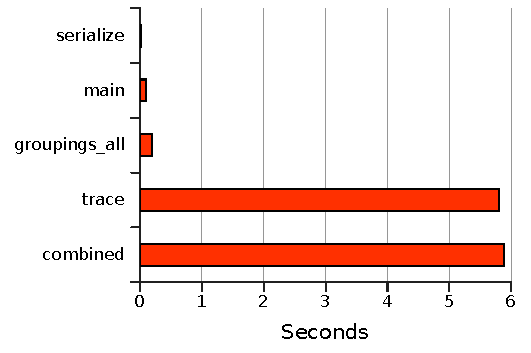
\includegraphics{optimizations/runtimes.pdf}
%%   \caption{Runtimes for the programs}
%%   \label{fig:runtimes}
%% \end{figure}
\subsubsection{Profiling}
We need to analyze the runtime behavior of the programs, to see which
functions takes up the runtime of the programs. For this purpose, we used a 
external tool, a profiler, of which there are many to chose from. We chose to use \texttt{gprof}
as it can give us an overview of which functions are called and how
much time is spent in each.

The programs was compiled and linked with the \texttt{-pg} option to
enable profiling data to be collected for \texttt{gprof}. We need to
extend the runtimes to get better results from \texttt{gprof}, so
instead of the text from \url{lipsum.com} we used a log file of
suitable size. The size was chosen to be small enough to fit in
memory, but big enough to produce longer runtimes. Section
\vref{sec:profiling.pl} contains the perl script used for 
profiling.

In figures \ref{fig:main_unoptimized},
\ref{fig:groupings_all_unoptimized}, \ref{fig:trace_unoptimized} and
\ref{fig:serialize_unoptimized} we have the output from
\texttt{gprof} flat profile column marked \texttt{\% time}. This
column describes the percentage of the total running time used by this
function. Only functions taking up more than 5\% of the total runtime
is included, the rest is bunched together in the other column.

\paragraph{\texttt{main}}
\begin{figure}
  \centering
  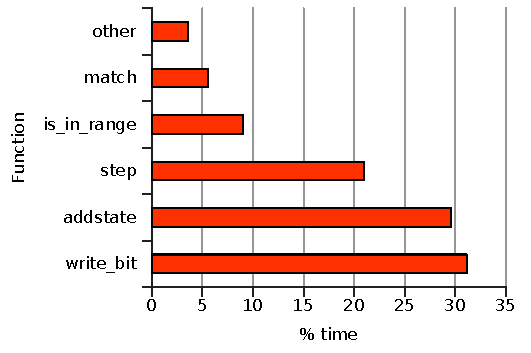
\includegraphics[]{optimizations/main_unoptimized.pdf}
  \caption{Output of \texttt{gprof} running \texttt{main}}
  \label{fig:main_unoptimized}
\end{figure}
In figure \vref{fig:main_unoptimized} we have the values for running
\texttt{main}. Functions \lstinline{add_state}, \lstinline{step},
\lstinline{is_in_range} and \lstinline{match} is all called in the
process of simulating the NFA, this takes up about 65\% of the total
runtime. The rest is taken up by IO: Function
\lstinline{write_bit}. For this example, the process of creating the
NFA is near instantaneous. We can also see the penalty for choosing a
simple solution to the character class problem, the function for
deciding membership \lstinline{is_in_range} takes up about 9\% of the
total runtime.

\paragraph{\texttt{groupings\_all}}
\begin{figure}
  \centering
  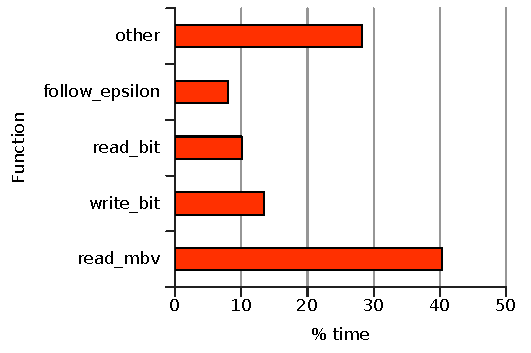
\includegraphics[]{optimizations/groupings_all_unoptimized.pdf}
  \caption{Output of \texttt{gprof} running \texttt{groupings\_all}}
  \label{fig:groupings_all_unoptimized}
\end{figure}
In figure \vref{fig:groupings_all_unoptimized} we have the values for
running \texttt{groupings\_all}. The main loop function,
\lstinline{read_mbv} takes up about 40\% of the total runtime. We also
see a large amount of runtime being taken up by functions with a small
amount of runtime each, these are helper functions to the main loop
and functions to do with keeping track of the channels. Again does the
IO functions \lstinline{write_bit} and \lstinline{read_bit} take up a
fair amount of runtime, about 23\%.

\paragraph{\texttt{trace}}
\begin{figure}
  \centering
  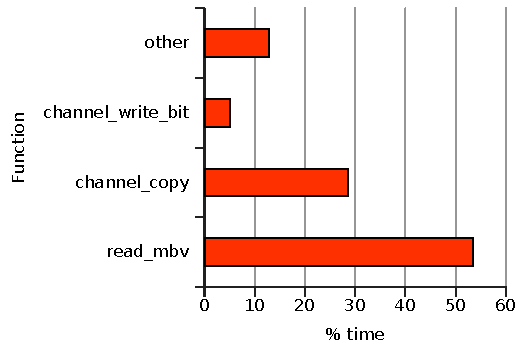
\includegraphics[]{optimizations/trace_unoptimized.pdf}
  \caption{Output of \texttt{gprof} running \texttt{trace}}
  \label{fig:trace_unoptimized}
\end{figure}
In figure \vref{fig:trace_unoptimized} we have the values for running
\texttt{trace}. The main loop function \lstinline{read_mbv} takes up
more than half the total runtime. We spend a lot of time copying,
writing to, appending and freeing channels, about 40\% of the total
runtime. Functions prepended with a \lstinline{channel_} deal with
channel management. Here the IO functions \lstinline{read_bit} and
\lstinline{write_bit} take up a relatively little amount of runtime,
about 5\% in total.

\paragraph{\texttt{serialize}}
\begin{figure}
  \centering
  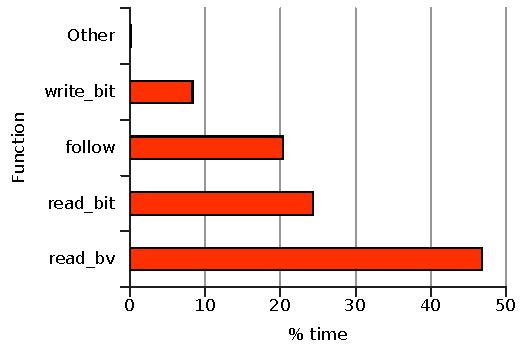
\includegraphics{optimizations/serialize_unoptimized.pdf}
  \caption{Output of \texttt{gprof} running \texttt{serialize}}
  \label{fig:serialize_unoptimized}
\end{figure}
In figure \vref{fig:serialize_unoptimized} we have the values for
running \texttt{serialize}. Again the main loop function takes up a
lot of time, about 47\% of the total runtime. I/O functions
\lstinline{read_bit} and \lstinline{write_bit} takes up about a third
of the total runtime.

\subsection{Applying the knowledge gained}

In the previous section we identified a few trouble spots and we will discuss potential remedies in this section. 
\begin{description}
\item[IO] From the output of \texttt{gprof} we can see that a lot of
  our runtime, in most programs, is used in the two I/O functions
  \lstinline{read_bit} and \lstinline{write_bit}.
\item[\texttt{trace}] \lstinline{trace} takes to long to complete, a
  good place to start would be to look for a way around all the
  channel management.
\item[Main loops] A lot of the runtime is spend in main loops. This is
  not necessarily a good place to start optimizing, this could just as
  well be because we were not good at spreading out the workload in
  smaller functions.
\end{description}


\subsubsection{$\upvarepsilon$-lookahead}

Each $\upvarepsilon$-transition is marked with a look-ahead
symbol. The $\upvarepsilon$-transition can then only be taken if the
look-ahead symbol matches the next character in the input string. This
optimization will have double effect, it will both reduce the number
of states in the active set when simulating the NFA and it will reduce
the mixed bit-values output at the cost of extra memory for and time
spend constructing the NFA.

This optimization has not been implemented.

\subsubsection{Improved protocol encoding}
The protocol used for transmitting data is text-based, using a binary
protocol would make the content more terse, but also nigh impossible
to read for a human. 

To transmit one operator in the text based protocol we always use 8
bits. Since we only have 8 different operators, this can be done using
less bits. A widely used and effective technique for lossless
compression of data is Huffman codes \cite{Cormen}. To encode our data
efficiently with Huffman codes we need to analyze our data; we need to
know the frequency with which the operators appear. In table
\vref{tab:huffman_freq} we have some frequencies of the operators
using different regular expressions on a text file generated by
\url{www.lipsum.org} of size 114KB. We have a simple and a somewhat
complex example. Since this is a table of operator frequencies, we
have left out the escaped characters, this means the numbers will not
sum to 100. What is missing is the escaped characters, these have the
same frequency as the escape operator.

\ctable[
  caption = Frequencies of operators in a mixed bit-value string,
  label = tab:huffman_freq
]{l|rr}{
  \tnote[a]{\textsf{.*}}
  \tnote[b]{\textsf{(?:(?:(?:[a-zA-Z]+ ?)+[,.;:] ?)*..)*}}
}{\FL
Operator & Match all\tmark[a] & Match words\tmark[b]\ML
\texttt{0} & 11\% & 13\% \NN
\texttt{1} & 11\% & 13\% \NN
\texttt{:} & 22\% & 27\% \NN
\texttt{\textbar} & 11\% & 2\% \NN
\texttt{=} & 11\% & 13\% \NN
\texttt{\textbackslash} & 11\% & 8\% \NN
\texttt{b} & 11\% & 13\% \NN
\texttt{t} & 0\% & 0\% \LL
}

In figures \vref{fig:huffman1} and \vref{fig:huffman2} we have the
corresponding Huffman trees, they yield the encoding in table
\vref{tab:huffman_codes}. We observe that as the regular expression
gets more complicated, we use \texttt{\textbar} and
\texttt{\textbackslash} less and \texttt{0}, \texttt{1}, \texttt{:},
\texttt{=} and \texttt{b} more. This is also reflected in the Huffman
encoding. Since most regular expression will be more complex than
\textsf{.*}, we choose the encoding in the match words column. This
gives us a compression ratio of 0.39, for the match words case
and a compression ratio of 0.44 for the match all case. 

\ctable[
  caption = Huffman encoding,
  label = tab:huffman_codes
]{l|rr}{
  \tnote[a]{\textsf{.*}}
  \tnote[b]{\textsf{(?:(?:(?:[a-zA-Z]+ ?)+[,.;:] ?)*..)*}}
}{\FL
Operator & Match all\tmark[a] & Match words\tmark[b]\ML
\texttt{0}              & 1110 & 010   \NN
\texttt{1}              & 010  & 110   \NN
\texttt{:}              & 00   & 10    \NN
\texttt{\textbar}       & 011  & 01110 \NN
\texttt{=}              & 100  & 111   \NN
\texttt{\textbackslash} & 101  & 0110  \NN
\texttt{b}              & 110  & 00    \NN
\texttt{t}              & 1111 & 01111 \LL
}

We can not make assumptions beforehand as to the frequencies of the
escaped characters. Their frequency depends highly on the text being
matched. If the escaped characters all have the same frequency, then
the Huffman method can achieve no compression. Instead we can look to
the character class that generated the escaped character. By rewriting
the character class with the \textsf{\textbar} operator and creating
the corresponding partial NFA as a balanced tree and use this tree as
we would a Huffman tree, we can compress the escaped characters. How
efficient this method is depends on how many characters is matched by
the character class. For example if we match all characters, then no
compression would be obtained, if on the other hand we had a small
character class like \textsf{[a-d]} we could encode characters matched
by this class using only 2 bits. 

We did not implement this optimization.

\subsubsection{Buffering input and output}

%% \begin{figure}
%%   \centering
%%   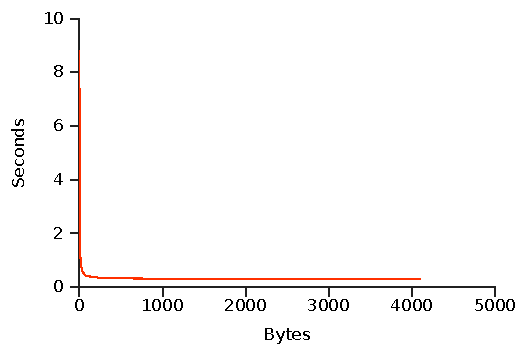
\includegraphics[]{optimizations/buffersize.pdf}
%%   \caption{Combined runtimes with different buffersize for input and output}
%%   \label{fig:buffersize}
%% \end{figure}
\ctable[
  caption = Runtimes for different buffersizes,
  label = tab:buffersize
]{rr|rr}{
}{\FL
Buffer size (B) & Runtime (s) & Buffer size (B) & Runtime (s)\ML
0   &   8.786 & 128 &	0.391\NN
2   &	4.507 & 256 &	0.338\NN
4   &	2.559 & 512 &	0.320\NN 
8   &	1.354 & 1024&	0.313\NN
16  &	0.886 & 2048&	0.314\NN
32  &	0.618 & 4096&	0.310\NN
64  &	0.437 & 8196&   0.324\LL
}

The two functions called when doing I/O is \lstinline{fputc} and
\lstinline{fgetc}. These are included with the \texttt{stdio.h} header
file. Reading up on those two reveal that they are buffered and
thread-safe. There is even a function for manipulating the buffering
method: \lstinline{setvbuf}. We did a bit of experimenting with
\lstinline{setvbuf}, the results are shown in figure
\vref{tab:buffersize}. The runtimes in the graph is the combined
runtime of all programs, i.e. we measured the runtime for all programs
combined with pipes:
\begin{verbatim}
echo lipsum | ./main regex | ./groupings_all regex  |  \
./trace | ./serialize regex'
\end{verbatim}
\texttt{regex} and \texttt{lipsum} are the same as used in section
\vref{sec:finding_out_where}. We can see that not much is gained from
a buffer size exceeding 1024 bytes.

\paragraph{Thread-safety}
We also looked into thread safety. There are non-thread-safe variants of
\lstinline{fputc} and \lstinline{fgetc}, \lstinline{fputc_unlocked}
and \lstinline{fgetc_unlocked} respectively. Note that the man-pages
does state that these thread-unsafe functions probably should not be
used. The results from an experiment similar to the previous, only
using the non-thread-safe functions for IO, are in table
\vref{tab:buffersize_unlocked}. The non-thread-safe functions are on
average 0.16\todo{jan: percentage would be better but this section is not that relevant} seconds faster. 

\ctable[
  caption = Runtimes for different buffersizes using non-thread-safe functions,
  label = tab:buffersize_unlocked
]{rr|rr}{
}{\FL
Buffer size (B) & Runtime (s) & Buffer size (B) & Runtime (s)\ML
0	&8.597 & 128	&0.248 \NN
2	&4.355 & 256	&0.204 \NN
4	&2.288 & 512	&0.181 \NN
8	&1.240 & 1024	&0.177 \NN
16	&0.716 & 2048	&0.164 \NN
32	&0.463 & 4096	&0.151 \NN
64	&0.308 & 8192	&0.162 \LL
}


%% Experimenting with the
%% \lstinline{setvbuf} function gave no improvement in runtimes. We can
%% also try looking into the threadsafety. There are thread-unsafe
%% variants of \lstinline{fputc} and \lstinline{fgetc},
%% \lstinline{fputc_unlocked} and \lstinline{fgetc_unlocked}
%% respectively. This gave some results, note that the man-pages does
%% state that these thread-unsafe functions probably should not be
%% used. We can also implement our own buffering mechanism and call
%% functions \lstinline{fputs} and \lstinline{fgets} instead. These two
%% functions read/write a whole line instead of a single character. This
%% also gave some results. 


\subsubsection{Channel management in \lstinline{trace}}

The problem with \lstinline{trace} is that we do not know which
channel has a match, so we need to keep track of the bit-values on all
of them. If we instead read the mixed bit-values backwards, the first
character we would read on a channel would be the \texttt{t} or
\texttt{b} operator, precluding the problem of knowing which channel
has a match. This does require us to read the whole string of mixed
bit-values and reversing it. Because this filter already is
non-streaming, it will not become a problem reading and storing the
whole string of mixed bit-values.

This optimization is implemented. Running the experiments determining
runtime and memory usage for the improved \texttt{trace} gives us a
runtime of just 1.309 seconds and a memory usage of 1536KB. Comparing
this to the values for the old \lstinline{trace} we see a huge
performance gain in runtime and a slight increase in memory
consumption. This optimization is well worth it.

We would expect no performance gain on this optimization when the
regular expression consists of a string of literals, that is we only
create one channel when simulating the NFA. This is however not a very
useful application of regular expressions, there are faster ways of
comparing two strings.

\clearpage
\section{Analysis of algorithms}
\label{sec:theoretical}
In this section we analyze the complexity of the various programs and
filters. We will not present pseudo code for the functions, it was not
within the capabilities of the authors to boil down 500+ lines of
C-code to half a page worth of orderly pseudo code. Instead we present
tables of functions, with a short description of what it does and what
other functions it calls and whether or not this is done in a
loop. Most importantly we will include the complexity of each function
in the tables. 

In the following sections $n$ denotes the length of the regular
expression and $m$ is the length of the input string.

\subsection{Constructing the NFA}

In tables \ref{tab:re2nfa1}, \ref{tab:re2nfa2} and \ref{tab:re2nfa3}
we have a overview of the functions involved in constructing a NFA. We
have the theoretical upper bound on run time and memory consumption in
big-o notation. Most functions are straightforward but a few deserve a
comment. 

\lstinline{ptrlist_patch} is the function that patches a list of
dangling pointers to a state. The pointers are only dangling once in
their lifetime, they do not become dangling again once they are
patched to a state. The upper bound on the total number of dangling
pointers is two times the number of states and the state count is
linear in the size of the regular expression, making the upper bound
on the number of pointers linear in the size of the regular expression
also. The total amount of work is linear in the size of the regular
expression. The number of times the \lstinline{ptrlist_patch} function
is called is linear in the size of the regular expression. The
amortized cost of calling the \lstinline{ptrlist_patch} function is
therefore O(1).

\lstinline{ptrlist_free}, see argument for \lstinline{ptrlist_patch}.

\lstinline{cc2fragment} also has a loop over the regular
expression. The reason why this does not become a O($n^2$) operation is
that the loop counter is shared between the two functions. Any
progress made by one function in the regular expression is shared with
the other.

We note that all functions called by the main loop function
\lstinline{re2nfa} are O(1) both in run time and memory, apart from
\lstinline{cc2fragment} see above comment. \lstinline{re2nfa}
allocates a stack for use in the construction process, the number of
elements in the stack is the number of characters in the regular
expression. We call the functions a number of times that are linear in
the size of the regular expression, we therefore conclude that
constructing a NFA is O($n$) in both run time and O($n$) in memory
consumption.

\ctable[
  caption = Analysis of \texttt{re2nfa} (part 1),
  label = tab:re2nfa1
]
{lp{5cm}cc}
{
  \tnote[a]{Amortized cost}
}
{\FL
  Function & Description & Run time & Memory \ML
  \lstinline{state} & Allocates memory for states & O(1) & O(1) \NN
  \lstinline{fragment} & Assigns values for a fragment & O(1) & O(1) \NN
  \lstinline{ptrlist_list1} & Allocates pointer list of one & O(1) &
  O(1) \NN
  \lstinline{ptrlist_patch} & Patches list of pointers & O(1)\tmark[a] & O(1)
  \NN
  \lstinline{ptrlist_append} & Appends two lists of pointers & O(1) &
  O(1) \NN
  \lstinline{ptrlist_free} & Frees list of pointers  &  O(1)\tmark[a]
  & O(1) \NN
  \lstinline{read_paren_type} & Determines parenthesis type & O(1) &
  O(1) \NN
  \lstinline{range} & Allocates memory for a range & O(1) & O(1) \NN
  \lstinline{parse_cc_char} & Parses a character in a character class
  & O(1) & O(1) \LL
}

\ctable[
  caption = Analysis of \texttt{re2nfa} (part 2),
  label = tab:re2nfa2
]
{lp{5cm}cc}
{
}
{\FL
  Function & Description & Run time & Memory \ML
  \lstinline{cc2fragment} & Makes a fragment of a character
  class. Calls \lstinline{state} and \lstinline{fragment} sequentially
  and \lstinline{parse_cc_range} in a loop over the regular expression
  & O(n) & O(1) \NN
  \lstinline{parse_cc_range} & Parses a range in a character
  class. Calls \lstinline{range} and \lstinline{parse_cc_char}
  sequentially  & O(1) & O(1) \NN
  \lstinline{maybe_concat} & Concatenates top two fragments. Calls
  \lstinline{ptrlist_patch} and \lstinline{ptrlist_free}
  sequentially & O(1) & O(1) \NN
  \lstinline{maybe_alternate} & Alternates top fragments. Calls
  \lstinline{state}, \lstinline{fragment}, \lstinline{ptrlist_list1} and
  \lstinline{ptrlist_append} sequentially & O(1) & O(1) \NN
  \lstinline{do_right_paren} & Does a right parenthesis. Calls
  \lstinline{maybe_concat}, \lstinline{maybe_alternate},
  \lstinline{state}, \lstinline{fragment} and
  \lstinline{ptrlist_list1} sequentially & O(1) & O(1) \NN
  \lstinline{finish_up_regex} & Finishing touches on forming the
  NFA. Calls \lstinline{state}, \lstinline{maybe_concat},
  \lstinline{maybe_alternate}, \lstinline{ptrlist_append},
  \lstinline{ptrlist_list1}, \lstinline{ptrlist_patch} and
  \lstinline{ptrlist_free} sequentially & O(1) & O(1) \NN
  \lstinline{do_quantifier} & Does quantifier. Calls
  \lstinline{state}, \lstinline{ptrlist_patch}, \lstinline{fragment},
  \lstinline{ptrlist_list1}, \lstinline{ptrlist_append}
  sequentially. & O(1) & O(1) \LL
}

\ctable[
  caption = Analysis of \texttt{re2nfa} (part 3),
  label = tab:re2nfa3
]
{lp{5cm}cc}
{
}
{\FL
  Function & Description & Run time & Memory \ML
  \lstinline{re2nfa} & Main loop. Calls \lstinline{state}, \lstinline{do_quantifier},
  \lstinline{maybe_concat}, \lstinline{maybe_alternate},
  \lstinline{fragment}, \lstinline{do_right_paren},
  \lstinline{cc2fragment} looping over the regular expression and
  \lstinline{finish_up_regex} sequentially & O(n) & O(n)
  \LL
}

\subsection{Simulating the NFA}

In table \ref{tab:match} we have the overview of functions involved in
the simulation of the NFA. We have the theoretical upper bound on run
time and memory consumption in big-O notation. Some functions deserve
a comment.

\lstinline{addstate} and \lstinline{last_addstate} marks states they
already have visited in one step. Upon encountering a state it already
has visited, it returns. This means that the total amount of work in a
single \lstinline{step} is O($n$) and not O($n^2$).

\lstinline{is_in_range} is also called once per active state in
\lstinline{step} and \lstinline{last_step}. We only create one state
per character class, what we do instead is create a list of ranges
representing the character class. The more ranges the fewer states and
vice versa. This (again) means that the total amount of work in a
single \lstinline{step} is O($n$) and not O($n^2$).

We note that for each character in the input string, in the worst case
we have to visit all states: O($n*m$). We allocate space enough for
the NFA which is O($n$) and two lists to keep track of the active
states which is also O($n$), resulting in a total of O($n$).

\ctable[
  caption = Analysis of \texttt{match},
  label = tab:match
]
{lp{5cm}cc}
{
}
{\FL
  Function & Description & Run time & Memory \ML
  \lstinline{is_in_range} & Determines if a character is accepted by a
  character class & O($n$) & O(1) \NN
  \lstinline{read_bit} & Reads character from input & O(1) & O(1) \NN
  \lstinline{write_bit} & Outputs bit & O(1) & O(1) \NN
  \lstinline{last_addstate} &  Add a state with final character in
  input string. Calls \lstinline{write_bit}
  \lstinline{last_addstate} & O($n$) & O(1) \NN 
  \lstinline{last_step} & Advance simulation final character. Calls
  \lstinline{last_addstate}, \lstinline{is_in_range} and \lstinline{write_bit} in a loop over
  active states & O($n$) & O(1) \NN
  \lstinline{addstate} & Add a state. Calls \lstinline{write_bit} and
  \lstinline{addstate} & O($n$) & O(1) \NN
  \lstinline{step} & Advances simulation one character. Calls
  \lstinline{addstate} and \lstinline{write_bit} in a loop over 
  active states & O($n$) & O($n$) \NN
  \lstinline{match} & Matches a NFA with a string & O($m*n$) & O($n$)
  \NN
  \LL
}

\subsection{The 'match' filter}

We see no reason for a table of functions for this filter, we only
call \lstinline{write_bit} and \lstinline{read_bit} once per input
character. This results in a run time linear in the input length and a
memory consumption of O(1).

\subsection{The 'groupings' filter} 

In table \ref{tab:groupings} we have the overview of the functions in
the 'groupings' filter, $o$ is the input length. 

\lstinline{follow_epsilon} follows all possible transitions for a
channel. The number of possible transitions is bounded the number of
actual transitions O($n$). No loops are entered, since these requires
a character from input. It is called virtually once for every input
character. This leads us to overall complexity for this filter:
O($n*o$). The memory used is the memory for the NFA and the list of
active channels, we cannot have more active channels than states:
O($n$).

\ctable[
  caption = Analysis of the 'groupings' filter,
  label = tab:groupings
]
{lp{5cm}cc}
{
}
{\FL
  Function & Description & Run time & Memory \ML
  \lstinline{channel} & Allocates memory for channel & O(1) & O(1) \NN
  \lstinline{channel_copy} & Copies a channel & O(1) & O(1) \NN
  \lstinline{channel_free} & Frees a channel & O(1) & O(1) \NN
  \lstinline{channel_remove} & Removes a channel from the channel
  list. Calls \lstinline{channel_free}
  & O(1) & O(1) \NN
  \lstinline{follow_epsilon} & Follow all possible transitions from
  current state. Calls \lstinline{write_bit} &
  O($n$) & O(1) \NN
  \lstinline{do_end} & Channel has ended. Calls
  \lstinline{channel_remove} and \lstinline{write_bit} & O(1) & O(1) \NN
  \lstinline{do_split} & Splits the channel. Calls
  \lstinline{channel_copy} & O(1) & O(1) \NN
  \lstinline{do_one} & Channel takes the transition marked 1. Calls
  \lstinline{write_bit} and \lstinline{follow_epsilon} & O($n$) & O(1) \NN
  \lstinline{do_zero} & Channel takes the transition marked 0. Calls
  \lstinline{write_bit} and \lstinline{follow_epsilon} & O($n$) & O(1) \NN
  \lstinline{do_escape} & Handles escaped character in input. Call
  \lstinline{follow_epsilon} and \lstinline{write_bit} & O($n$) & O(1)
  \NN
  \lstinline{read_mbv} & Main loop. Calls \lstinline{read_bit},
  \lstinline{write_bit}, \lstinline{do_split}, \lstinline{do_end},
  \lstinline{do_zero}, \lstinline{do_one}, \lstinline{do_escape} in a loop over the input and
  \lstinline{follow_epsilon} & O($n*o$) & O($n$) \NN
  \lstinline{main} & Calls \lstinline{re2nfa} and \lstinline{read_mbv}
  & O($n*o$) & O($n$)
  \LL
}


\subsection{The 'trace' filter} 

In table \ref{tab:trace} we have the overview of the functions in the
trace' filter, $o$ is the input length. The version of the 'trace'
filter analyzed here, is the optimized one.

\lstinline{channel_write_bit} reallocates memory when it runs out, the
allocation strategy is to double the amount of memory every time we
run out. The complexity of copying the data over all calls to
\lstinline{channel_write_bit} is 1 + 2 + 4 + 8 + ... $o$ =
O($o$). Because this is the cost of all calls to
\lstinline{channel_write_bit}, the cost of \lstinline{trace} is only
O($o$) and not O($o^2$).

This filter is O($o$) complexity both in run time and memory. 

\ctable[
  caption = Analysis of the 'trace' filter,
  label = tab:trace
]
{lp{5cm}cc}
{
}
{\FL
  Function & Description & Run time & Memory \ML
  \lstinline{channel_write_bit} & Writes bit in channel. Reallocates
  memory if necessary & O($o$) & O($o$) \NN
  \lstinline{trace} & Reads mixed bit-values backwards and stores the
  channel containing a match. Calls \lstinline{channel_write_bit} in a
  loop over the mixed bit-values & O($o$) & O($o$) \NN
  \lstinline{read_mbv} & Reads whole input string into memory,
  reallocates memory if it runs out. Calls
  \lstinline{read_bit} in a loop over input & O($o$) & O($o$) \NN
  \lstinline{reverse} & Reverses input string & O($o$) & O($o$) \NN
  \lstinline{main} & Calls \lstinline{read_mbv}, \lstinline{reverse},
  \lstinline{trace} and \lstinline{write_bit} & O($o$) & O($o$) \NN
  \LL
}


\subsection{The 'serialize' filter}

In table \ref{tab:serialize} we have the functions in the 'serialize'
filter. $o$ is the input length. 

This is not a complicated filter. We basically just read input and
step through the NFA: O($o*n$). The only memory we allocate is for the
NFA: O($n$).


\ctable[
  caption = Analysis of the 'serialize filter,
  label = tab:serialize
]
{lp{5cm}cc}
{
}
{\FL
  Function & Description & Run time & Memory \ML
  \lstinline{follow} & Follows all legal transitions. Calls \lstinline{write_bit} & O($n$) & O(1)
  \NN
  \lstinline{read_bv} & Reads bit-values from input. Calls
  \lstinline{read_bit}, \lstinline{write_bit} and \lstinline{follow} in a loop over input &
  O($o*n$) & O(1) \NN
  \lstinline{main} & Calls \lstinline{re2nfa} and \lstinline{read_bv}
  & O($o*n$) & O($n$) 
  \LL
}

\clearpage
\section{Evaluation}
\label{sec:evaluation}
In this section we will be looking at how our programs compare to
other implementations. We have chosen a few languages and libraries
that we feel are interesting:
\begin{description}
  \item[RE2] RE2 is a new open source library for C++ written by Russ
    Cox. It is only a little more than a year old. It uses automata
    when matching. It does not offer back-references.
  \item[TCL]
    TCL added regular expression support in a release in 1999. The
    regular expression engine is written by Henry Spencer. It uses a
    hybrid engine. It is a interpreted language.
  \item[Perl] Perl is from 1987 and is written by Larry Wall. It uses
    backtracking and virtual machines when matching. It is an
    interpreted language. 
\end{description}
They are few in numbers, but they cover the basics in underlying
technology and performance. 

The benchmarks here can not be considered exhaustive, instead we have
tried picking a few that would show interesting features of our
programs. Our implementation will be denoted as Main in
the graphs.

\paragraph{Input method}
Our chosen method of input has a drawback, namely the upper limit on
size for command line input. The system we tested on, see also
\vref{sec:specs}, has a upper limit on command line input of 2MB. This
can be ascertained (on our test system at least) by issuing the
following command:
\begin{verbatim}
$ getconf ARG_MAX
2097152
\end{verbatim}
In the unlikely event that a user will need to match with a regular
expression exceeding this 2MB limit, there is always the option to use
a file instead. Files only suffer the limit that they, along with the intermediate data generated by this solution, need to fit in
the free virtual memory space.

\subsection{A backtracking worst-case}

Our first benchmark is taken from \cite{RussCox} and demonstrates the
worst-case behavior of the backtracking algorithm. Using superscripts
to denote string repetition, we will be matching \textsf{a?$^n$a$^n$}
with the string \textsl{a$^n$}. For example will \textsf{a?$^3$a$^3$}
translate to \textsf{a?a?a?aaa}. We expect Perl to do poorly in this
benchmark, while the rest should do well.

For this experiment we used the programs \texttt{main} and
\texttt{ismatch}. The script used for the backtracking worst case is
in sections \vref{sec:backtrackingworstcase.pl} and
\vref{sec:backtrackingworstcase_mem.pl}.

\subsubsection*{Runtimes}

\begin{figure}
\centering
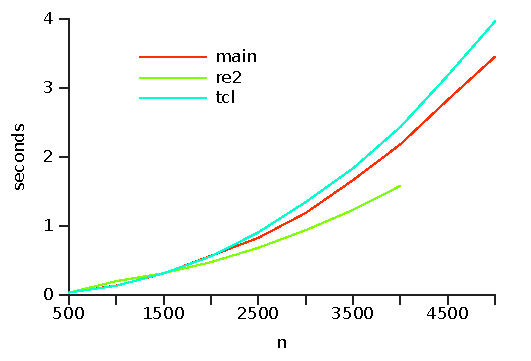
\includegraphics{benchmarks/backtrackingworstcase_maintclre2_normal.pdf}
\caption{A backtracking worst-case: Main, Tcl and RE2 runtimes.}
\label{fig:backtrackingworstcase_maintclre2_normal}
\end{figure}

\begin{figure}
\centering
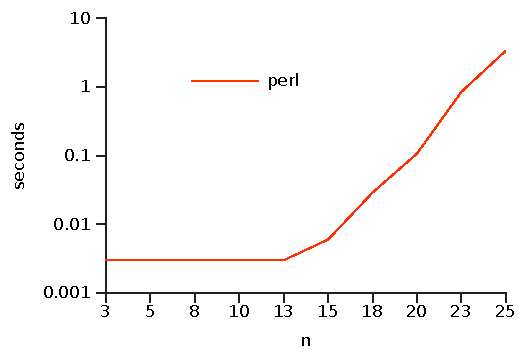
\includegraphics{benchmarks/backtrackingworstcase_perl_log.pdf}
\caption{A backtracking worst-case: Perl runtime on a logarithmic scale.}
\label{fig:backtrackingworstcase_perl_log}
\end{figure}

The runtimes can be seen in figures
\ref{fig:backtrackingworstcase_maintclre2_normal} and
\ref{fig:backtrackingworstcase_perl_log}. As anticipated: Perl
exhibits very poor performance. The slope on figure
\vref{fig:backtrackingworstcase_perl_log} and the logarithmic scale
suggest that Perl runs in time exponential in $n$. This is not
surprising considering that the \textsf{?} matches greedily,
meaning it will first try to consume a character from input. The only
way that the regular expression matches the string is if all the
quantifiers consume no input. There are $2^n$ possible ways for the
quantifiers to consume and not consume a character. The backtracking
engine has to search through all the $2^n$ possible solutions to find
the matching one, since it matches greedily.

In figure \vref{fig:backtrackingworstcase_maintclre2_normal} we do not
see much difference in the performance of Main, RE2 and Tcl. RE2 stops
before the others, it has a upper limit on how much memory it will
consume. The limit is user (compile time) defined for RE2. This limit
could have been set to a value that would allow RE2 to continue
matching with Main and Tcl. We chose not to do this, because we wanted
to demonstrate this feature in RE2. This feature is especially useful
in setups where memory is very tight or you accept regular expressions
from untrusted sources, but can obviously also be considered a
nuisance in other situations where you do not want to fiddle with this
limit, but just want to make RE2 do your matches.

As a side note, we found that if we added a literal \textsf{b} at the
end of the regular expression, so that the regular expression no
longer matches the string, we would suddenly see marked improvements
in the runtimes of Perl. Using a backtracking algorithm it would still
take time exponential in $n$ to decide they did not match, but Perl
scans the input string for all literals in the regular expressions,
and it quickly discovers that there is no \textsl{b} in the input
string, so therefore the regular expression can not match the string.

\subsubsection*{Memory usage}

\begin{figure}
\centering
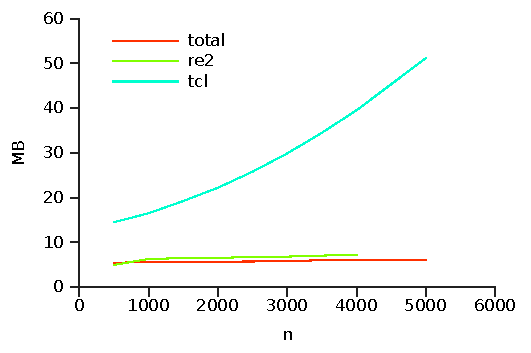
\includegraphics{benchmarks/memory/backtrackingworstcase_mem_totalre2tcl.pdf}
\caption{A backtracking worst-case: Total, Tcl and RE2 memory usage.}
\label{fig:backtrackingworstcase_mem_maintclre2_normal}
\end{figure}

\begin{figure}
\centering
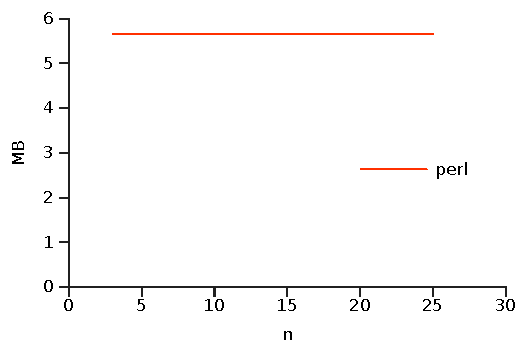
\includegraphics{benchmarks/memory/backtrackingworstcase_mem_perl.pdf}
\caption{A backtracking worst-case: Perl memory usage.}
\label{fig:backtrackingworstcase_mem_perl_log}
\end{figure}

Memory usage is depicted in figures
\ref{fig:backtrackingworstcase_mem_maintclre2_normal} and
\ref{fig:backtrackingworstcase_mem_perl_log}. For our program we have
added up the memory usage of the individual programs and displayed
them under the total header. 

In figure \vref{fig:backtrackingworstcase_mem_maintclre2_normal} we
again note that RE2 stops before the other two because of memory limitations. The memory usage of our programs and RE2 does not appear
to be more than linear in the input size, while Tcl looks more like some
quadratic function. It is hard to give a good explanation to this
without knowing Tcls' regular expression engine better; even if it did use a
NFA for this match, the size should still be linear in the input. Tcl
has the same asymptotic runtime performance as Main and RE2, but with
bigger constants; all that extra memory spent is not being put to
good use. 

Figure \vref{fig:backtrackingworstcase_mem_perl_log} shows Perls
memory usage. It is hard to say anything useful based on that graph,
the values for $n$ are too small. Unfortunately, due to the
exponential run-time of the problem it is not viable to increase them.

\subsection{A DFA worst-case}

Using superscripts to denote string repetition, constructing a DFA
from the regular expression \textsf{(a\textbar b)*a(a\textbar b)$^n$}
results in a exponential blow up of the state count. For example will
\textsf{(a\textbar b)*a(a\textbar b)$^3$} translate to
\textsf{(a\textbar b)*a(a\textbar b)(a\textbar b)(a\textbar
  b)}. Acceptance with a DFA is decided in time linear to the size of
the input string, but we would still have to store the DFA which takes
space exponential in the size of the regular expression. We expect any
regular expression engine using DFAs to do poorly on this
benchmark. The engines that can be expected to use DFAs are RE2 and
Tcl, but both can switch method according to need. 


For this experiment we used the programs \texttt{main} and
\texttt{ismatch}. The script used for the backtracking worst case is
in sections \vref{sec:dfaworstcase.pl} and
\vref{sec:dfaworstcase_mem.pl}.


\subsubsection*{Runtimes}

\begin{figure}
\centering
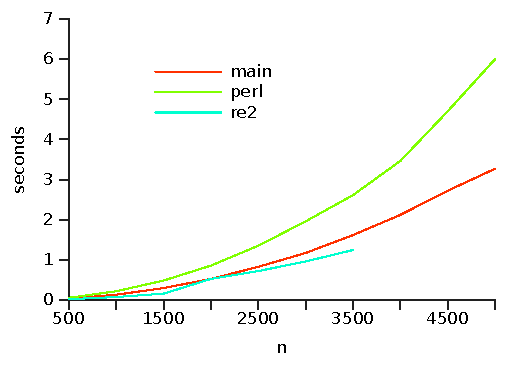
\includegraphics{benchmarks/dfaworstcase_mainre2perl_normal.pdf}
\caption{A DFA worst-case: Main, RE2 and Perl runtimes.}
\label{fig:dfaworstcase_mainre2perl_normal}
\end{figure}

\begin{figure}
\centering
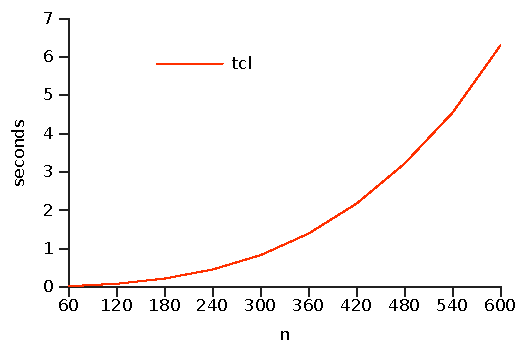
\includegraphics{benchmarks/dfaworstcase_tcl_normal.pdf}
\caption{A DFA worst-case: Tcl runtimes.}
\label{fig:dfaworstcase_tcl_normal}
\end{figure}

In figures \ref{fig:dfaworstcase_mainre2perl_normal} and
\ref{fig:dfaworstcase_tcl_normal} we have the figures displaying the
runtimes of the various programs. Again we note that RE2 stops before
the others, see above. Tcl stands out with significantly lower
performance, but none appears to have exponential or worse asymptotic
behavior. This would suggest that Tcl chooses to use a DFA in some
form for this match and RE2 falls back on something else.


\subsubsection*{Memory usage}

\begin{figure}
\centering
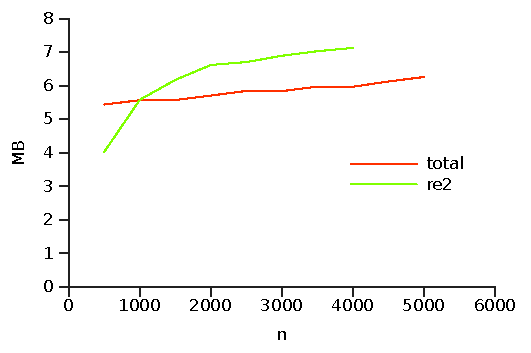
\includegraphics{benchmarks/memory/dfaworstcase_mainre2.pdf}
\caption{A DFA worst-case: Main and RE2 memory usage.}
\label{fig:dfaworstcase_mem_mainre2}
\end{figure}

\begin{figure}
\centering
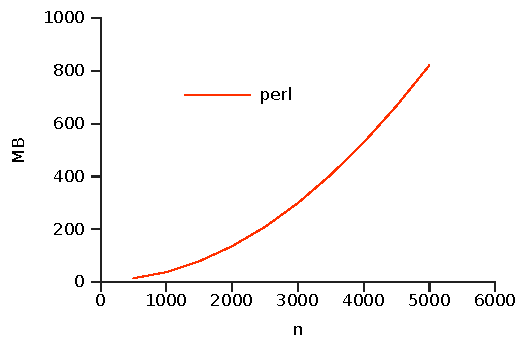
\includegraphics{benchmarks/memory/dfaworstcase_perl.pdf}
\caption{A DFA worst-case: Perl memory usage.}
\label{fig:dfaworstcase_mem_perl}
\end{figure}

\begin{figure}
\centering
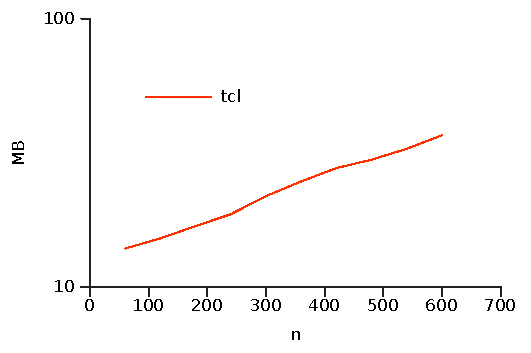
\includegraphics{benchmarks/memory/dfaworstcase_tcl_log.pdf}
\caption{A DFA worst-case: Tcl memory usage.}
\label{fig:dfaworstcase_mem_tcl_log}
\end{figure}

The memory usage proved to be a more complicated matter than the
runtimes, see figures \ref{fig:dfaworstcase_mem_mainre2},
\ref{fig:dfaworstcase_mem_perl} and \ref{fig:dfaworstcase_mem_tcl_log}
display.

Our programs and RE2 appears to be using memory linear in the size of
the regular expression. There is a sharp rise in memory consumed by
RE2 for $n$ smaller than about 1000. This would indicate that RE2 uses
a DFA until the exponential factor becomes to big and forces it to
switch method. 

Perls memory usage is mapped in figure
\vref{fig:dfaworstcase_mem_perl}. Compared to our programs Perl uses
rather a lot of memory. It seems to be increasing in a quadratic
manner.%\todo{investigate further}

In figure \vref{fig:dfaworstcase_mem_tcl_log} we have Tcls memory
usage mapped. Note the logarithmic scale. Our suspicion that Tcl uses
a DFA is confirmed by the memory usage, which appears to be
exponential in the size of the regular expression. 


\subsection{Extracting an email-address}

This is the first of our real world benchmarks. We will be extracting
an email-address from a string of text. Since we can not do partial
matches, we will be constructing strings of increasingly long
email-addresses. The regular expression is taken from
\cite{veanes}. Unlike the two previous benchmarks, the regular
expression is kept constant and does not grow.

Since we are extracting a value we are using \texttt{main},
\texttt{groupings\_all}, \texttt{trace} and \texttt{serialize} for
this match. The scripts can be found in sections \vref{sec:email.pl},
\vref{sec:email_mem.pl} and \vref{sec:email_mbvsize.pl}

\subsubsection*{Runtimes}

\begin{figure}
\centering
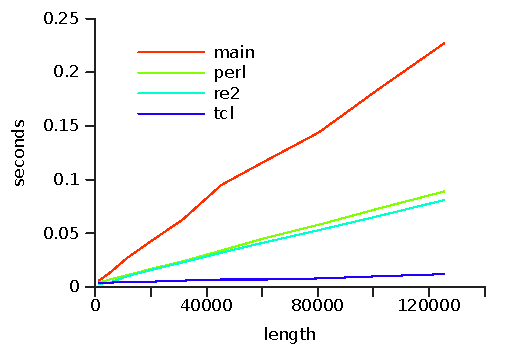
\includegraphics{benchmarks/email.pdf}
\caption{Extracting an email-address: Runtimes.}
\label{fig:email}
\end{figure}

In figure \vref{fig:email} contains the runtimes. All appear to be
running in time linear to the input string, with Tcl clearly having
the lowest constants and our programs the largest. 


\subsubsection*{Memory usage}
\begin{figure}
\centering
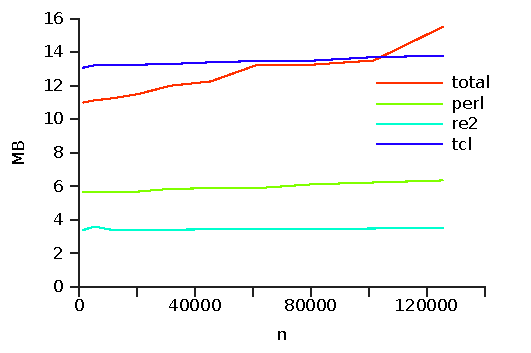
\includegraphics{benchmarks/memory/email_mem.pdf}
\caption{Extracting an email-address: Memory usage.}
\label{fig:email_mem}
\end{figure}

\begin{figure}
\centering
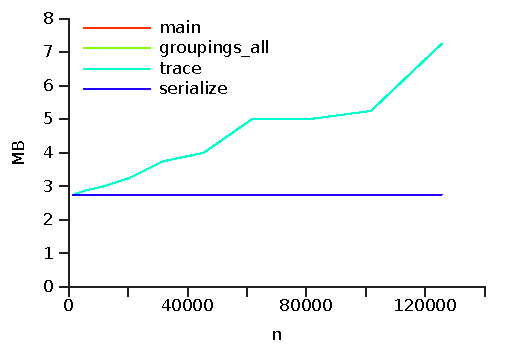
\includegraphics{benchmarks/memory/email_mem_individual.pdf}
\caption{Extracting an email-address: Individual programs memory usage.}
\label{fig:email_individual_mem}
\end{figure}

\begin{figure}
\centering
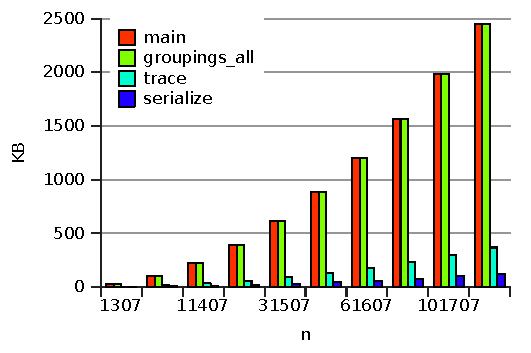
\includegraphics{benchmarks/memory/email_mbvsize.pdf}
\caption{Extracting an email-address: Sizes of output from individual
  programs.}
\label{fig:email_mbvsize}
\end{figure}


\begin{figure}
\centering
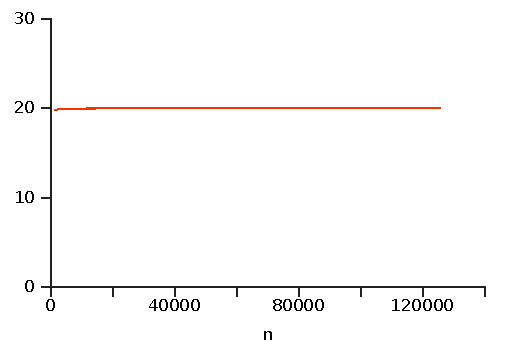
\includegraphics{benchmarks/memory/email_mbvsize_relative.pdf}
\caption{Extracting an email-address: The relationship between input
  size to \texttt{trace} and size of input string.}
\label{fig:email_mbvsize_relative}
\end{figure}


In figure \vref{fig:email_mem} we have the memory usage of the
programs. All programs except ours seem to be using memory linear in
the input string. We seem to be using memory in a stepped manner. This
correlates well with our scheme for memory management in
\texttt{trace}: We double the amount of memory used every time we run
out. This is confirmed by figure \vref{fig:email_individual_mem},
which displays the memory usage for the individual programs. Here we
see that all our programs except \texttt{trace} use a constant amount
of memory. It is hard to tell from figures
\ref{fig:email_individual_mem} and \vref{fig:email_mem} if the memory
used is linear in the input string. What we need to know is the size
of the mixed bit-values compared to the input string; we have
displayed this in figure \vref{fig:email_mbvsize} where we have the sizes
of the output from the individual programs. We did not put in a
separate column for the size of the input string since this is
exactly the same as the size of the output from
\texttt{serialize}. There is a linear relationship between the output
of \texttt{groupings\_all} and \texttt{serialize}: The first is 20
times bigger than the latter. See figure
\vref{fig:email_mbvsize_relative}.

\subsection{Extracting a number}

Our fourth and last benchmark is also a real world example taken from
\cite{veanes}. This one extracts a number from a string. We can not do
partial matches, so again we will be using a string consisting of
increasingly large numbers. The regular expression is constant.

We will be extracting a number, so we will be using programs
\texttt{main}, \texttt{groupings\_all}, \texttt{trace} and
\texttt{serialize} for this match. The scripts can be found in
sections \vref{sec:number.pl}, \vref{sec:number_mem.pl} and
\vref{sec:number_mbvsize.pl}.


\subsubsection*{Runtimes}

\begin{figure}
\centering
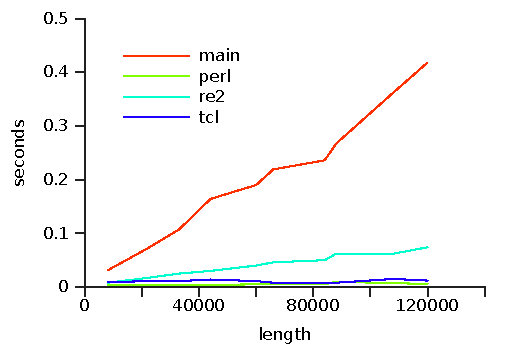
\includegraphics{benchmarks/number.pdf}
\caption{Extracting a number: Runtimes.}
\label{fig:number}
\end{figure}

In figure \vref{fig:number} we have the runtimes for this
benchmark. They all appear to be linear in the size of the input
string. Our programs clearly have bigger constants than the rest. 


\subsubsection*{Memory usage}


\begin{figure}
\centering
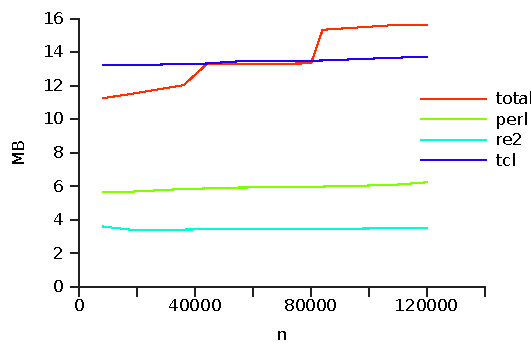
\includegraphics{benchmarks/memory/number_all.pdf}
\caption{Extracting a number: Memory usage.}
\label{fig:number_mem}
\end{figure}


\begin{figure}
\centering
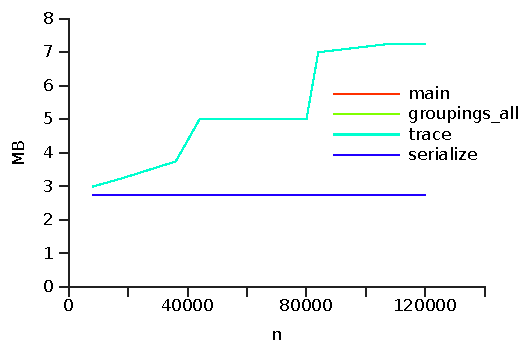
\includegraphics{benchmarks/memory/number_individual.pdf}
\caption{Extracting a number: Individual programs memory usage.}
\label{fig:number_mem_individual}
\end{figure}

\begin{figure}
\centering
\includegraphics{benchmarks/memory/number_mbvsize.pdf}
\caption{Extracting a number: Sizes of output from individual programs.}
\label{fig:number_mem_mbvsize}
\end{figure}


\begin{figure}
\centering
\includegraphics{benchmarks/memory/number_mbvsize_relative.pdf}
\caption{Extracting a number: The relationship between input size to
  \texttt{trace} and size of input string.}
\label{fig:number_mem_mbvsize_relative}
\end{figure}


In figure \vref{fig:number_mem} we have the memory usage. We clearly see the same pattern as in the extracting an
email address benchmark: that our programs use memory in a stepped but linear
manner and the rest use memory linear in the size of the input
string. We investigate further, see figure
\vref{fig:number_mem_individual} for the individual programs memory
usage. All our programs, except \texttt{trace} use a constant amount
of memory. The steps in the memory usage of \texttt{trace} is even
more pronounced in this figure. See above note on memory management
strategy in \texttt{trace} for explanation. The relationship between
the sizes of the output from the different programs is displayed in
figure \vref{fig:number_mem_mbvsize}. The size of the input string is
exactly the same as the output from \texttt{serialize}. For greater
clarity we have the relationship between the input size to
\texttt{trace} and the size of the input string displayed in figure
\vref{fig:number_mem_mbvsize_relative}. We do not observe the same
fixed relationship between the two as we did in the extracting an
email address benchmark - there seem to be no increasing trend. We
generate between 20 and 30 mixed bit-values per byte in the input
string.


\subsection{Large files}

We also did some experiments involving a large (333.5MB) log file. The
log file was lifted from another project where it was used to gather
data on file access \cite{jan2010}. The data in the log file was
aggregated, one line at a time, using some regular expressions that
could easily be translated for use in our regular expression
engine. Our experiment consisted of replicating the aggregation of
data. This is where our problems with this experiment began: We tried
to read the whole file at the same time, since the current version of our framework has no support for line-by-line reads. 
After some time this resulted in an out of memory error. 

This is not a problem specific for our framework; we observe that this operation on some
other existing implementation, such as Perl, also results in an out of
memory error. 

The lesson in this experiment is that we lack some way of applying
regular expression one line at a time. We could have tried applying
the regular expressions with the help of \texttt{awk}, but it seemed
superfluous invoking our pipeline of programs when \texttt{awk}
already has a perfectly good regular expression engine built in. Our
other choice would have been making a shell-script and used a loop and
\texttt{cat}. 

\subsection{Correctness}

We have to the best of our ability tested the programs for errors. 

This was accomplished by creating a large database of approximately 320+ test cases and repeatedly verifying the programs against this database, both during development and subsequent optimizations and changes. 

Unfortunately, it was discovered late in the project that a specific situation is not handled correctly. The problem has been fixed at the design level but is still present in the implementation: using the 'groupings' filter with a quantifier will not always
produce correct results, for example \textsf{(a)*} matched with
\textsl{aaa} will produce the output \texttt{111} from the
\lstinline{groupings_all} filter, which is not correct. Part of the
problem is that we are not producing the required bit-values to bind
the captured bit-values together.

\subsection{Conclusion}

We observe that our programs do not suffer from either the
backtracking worst-case or the DFA worst-case problems.

\paragraph{Correctness} We do not in all situations produce correct
output on all combinations of regular expressions, input strings and
filters. See example in section above.

\paragraph{Simple acceptance} We can compete on even footing with the
best when it comes to a simple acceptance decision. Our main program
combined with the 'match' filter is fast and uses memory linear in the
size of the regular expression.

\paragraph{Capturing groups} When it comes to the more complicated
task of capturing the contents of groups, we are lagging behind. The
task of capturing groups is achieved by a 4 programs long pipe in our
framework. Even if all of them only used memory linear in the length
of the regular expression, the overhead of running separate programs
add up.  The 'trace' filter uses memory linear in the size of the
input string. While this is obviously not quite as good as the other
filters, it is nevertheless a good result, we have managed to separate
this functionality into an independent component.

An obvious drawback is the constant basic overhead of having four
individual programs instead of one. We note however that this is
currently completely unoptimized and that this cost will not rise
relative to either input. It is also still quite low; it would likely only be a relevant problem in a demanding environment
such as embedded devices.

The other main problem is the blow up of the size of the mixed
bit-values. We have previously discussed potential solutions to this
problem.

\clearpage
\section{Related work}
\label{sec:related}
%% \todo[inline]{Opsummer hvad vi har haft af related work i rapporten of
%% inkluder det der ikke passede ind}

The groundwork of regular expression has been known for
decades. Current research is often focused generally; for
example to improve matching speeds, but there is also heavy activity
towards more specialized purposes, such as XML parsers, hardware based spam
detection or even such fields as biology where regular expressions are
often used to find patterns of amino acids. 

The intended aim of this particular project is towards the general
realm (the curios reader may wish to read \cite{pedersen2010} if they
are interested in special usages of regular expressions). For this
reason, the remainder of this section will therefore concentrate on
likewise general research.

%\todo{blah blah om ting du ikke har snakket naermere om}


\subsection{Constructing NFAs}

It is possible to construct different NFAs accepting the same
language. These NFAs will have different properties. 

%\todo[inline]{Find out other methods for constructing NFAs}

\subsection{Simulating NFAs}

\subsubsection{Frisch and Cardelli}

Frisch and Cardelli presents a method to simulate a NFA in their paper
\cite{2004:GreedyRegularExpressionMatching}. It works in two passes
over the input string. 

The first pass annotates the input string with
enough information to decide which branch to pick in alternations and
how many times to iterate a quantifier. This is done by reading the
input from right-to-left and working our way backwards in the NFA, the
visited states are annotated and stored with the input string. In the
second and main pass, where we read the input string left-to-right and
work our forwards in the NFA, these annotations are used to decide
which branch to take in an alternation and how many times to iterate a
star. This method is not suitable for a streaming regular expression
engine. The input string is read first from end-to-front and then from
front-to-end, this can not be done without storing the string.

\subsubsection{Backtracking}
Backtracking is a way of simulating a NFA. It is the method employed
by many programming languages and libraries, such as Perl and
PCRE. Compared to other methods, this has the advantage of allowing
backreferences, but it is also a worst-case exponential-time
algorithm. An example of a matching that exhibits worst-case behavior
is the regular expression \textsf{a?$^n$a$^n$} and the string
\textsl{a$^n$}, where superscripts denotes string repetition. This
example is also known from the article \cite{RussCox}.

A backtracking algorithm works depth-first. It has one active state
(\texttt{AS}) and a string pointer (\texttt{SP}) and a stack of
save-points. Every time we have to make a choice as to which
transition to take when traversing the NFA, we save the state so we
can later return and explore the alternate routes. Each save-point
consists of a state and a pointer to the string.

\begin{example}[Backtracking]
\begin{figure}
  \centering 
  \includegraphics{relatedwork/backtracking.pdf}
  \caption{NFA for \textsf{a*}}
  \label{fig:backtracking}
\end{figure}
In this example we will be matching \textsf{a*} to the string
\textsl{aa}. The NFA we will be using for this example is in figure
\vref{fig:backtracking}. The process of matching could look like:
\begin{center}
\begin{tabular}{cccp{7.5cm}}
  \texttt{AS} & \texttt{SP} & Save-points & Explanation \\ 

  \hline 

  1 & \textsl{\underline{a}a} &
  \rowcolors[\hline]{1}{lightgray}{lightgray}
  \begin{tabular}{c}
    \\
  \end{tabular} 
  & Initially \texttt{AS} is set to the start state and \texttt{SP} is
  set to the first character in the string\\
  
  2 & \textsl{\underline{a}a} & 
  \rowcolors[\hline]{1}{lightgray}{lightgray}
  \begin{tabular}{c}
    (1, \textsl{\underline{a}a})\\
  \end{tabular} 
  & Two paths are available, so we save the state and take the
  $\upvarepsilon$-transition to state 2. \\

  1 & \textsl{a\underline{a}} & 
  \rowcolors[\hline]{1}{lightgray}{lightgray}
  \begin{tabular}{c}
    (1, \textsl{\underline{a}a})\\
  \end{tabular} 
  & We take the transition back to state 1 and consume the first
  \textsl{a}. \\

  2 & \textsl{a\underline{a}} & 
  \rowcolors[\hline]{1}{lightgray}{lightgray}
  \begin{tabular}{c}
    (1, \textsl{\underline{a}a}) \\
    (1, \textsl{a\underline{a}})\\
  \end{tabular} 
  & Two paths are available, so we save the state and take the
  $\upvarepsilon$-transition to state 2. \\
  
  1 & \textsl{aa\underline{ }} &
  \rowcolors[\hline]{1}{lightgray}{lightgray}
  \begin{tabular}{c}
    (1, \textsl{\underline{a}a}) \\
    (1, \textsl{a\underline{a}})\\
  \end{tabular} 
  & We take the transition back to state 1 and consume the second
  \textsl{a}. \\

  2 & \textsl{aa\underline{ }} & 
  \rowcolors[\hline]{1}{lightgray}{lightgray}
  \begin{tabular}{c}
    (1, \textsl{\underline{a}a}) \\
    (1, \textsl{a\underline{a}}) \\
    (1, \textsl{aa\underline{ }})
  \end{tabular} 
  & Two paths are available, so we save the state and take the
  $\upvarepsilon$-transition to state 2. \\
  
  \\

  1 & \textsl{\underline{a}a} &   
  \rowcolors[\hline]{1}{lightgray}{lightgray}
  \begin{tabular}{c}
    (1, \textsl{a\underline{a}}) \\
    (1, \textsl{aa\underline{ }})
  \end{tabular} 
  & No transitions are available from state 2, so this path is
  abandoned. We backtrack and pop a save-state. \\
  
  3 & \textsl{\underline{a}a} &   
  \rowcolors[\hline]{1}{lightgray}{lightgray}
  \begin{tabular}{c}
    (1, \textsl{a\underline{a}}) \\
    (1, \textsl{aa\underline{ }})
  \end{tabular} 
  & The other available $\upvarepsilon$-transition to state 3 is
  taken. \\

  1 & \textsl{a\underline{a}} &   
  \rowcolors[\hline]{1}{lightgray}{lightgray}
  \begin{tabular}{c}
    (1, \textsl{aa\underline{ }})
  \end{tabular} 
  & No transitions are available from state 3, so this path is
  abandoned. We backtrack and pop a save-state. \\
  
  3 & \textsl{a\underline{a}} &   
  \rowcolors[\hline]{1}{lightgray}{lightgray}
  \begin{tabular}{c}
    (1, \textsl{aa\underline{ }})
  \end{tabular} 
  & The other available $\upvarepsilon$-transition to state 3 is
  taken. \\

  1 & \textsl{aa\underline{}} &
  \rowcolors[\hline]{1}{lightgray}{lightgray}
  \begin{tabular}{c}
    \\
  \end{tabular} 
  & No transitions are available from state 3, so this path is
  abandoned. We backtrack and pop a save-state. \\

  
  3 & \textsl{a\underline{a}} &
  \rowcolors[\hline]{1}{lightgray}{lightgray}
  \begin{tabular}{c}
    \\
  \end{tabular} 
  & The other available $\upvarepsilon$-transition to state 3 is
  taken. We have reached the end of the string and are in an accepting
  state: We have a match! \\
\end{tabular}
\end{center}
\end{example}


\subsection{Virtual machine}
Another popular method of matching regular expressions to text is the
virtual machine approach \cite{Cox2009}. Instead of constructing a
automaton, we generate byte-code for an interpreter. 

A simple virtual machine would have the ability to execute threads,
each thread consisting of a regular expression program. Each thread
would maintain a program counter (\texttt{PC}) and a string pointer
(\texttt{SP}). A regular expression program could for example consist of
the following instructions:
\begin{description}
\item[\texttt{char} $c$] If the \texttt{SP} does not point to a $c$
  character, then this thread of execution is abandoned. Otherwise,
  the \texttt{SP} and the \texttt{PC} is advanced.
\item[\texttt{match}] Stop thread, we have a match.
\item[\texttt{jmp} $x$] \texttt{PC} is set to $x$.
\item[\texttt{split} $x$\texttt{,} $y$] Split the thread of execution. The new
  threads \texttt{PC} is set to $x$ and the old threads \texttt{PC} is
  set to $y$.
\end{description}
With these few and simple instructions we are able to compile regular
expressions with concatenation, alternation and repetition, see table
\vref{tab:code_sequences}. 
\ctable[
  caption = Code sequences,
  label = tab:code_sequences
]
{lll}
{}
{\FL
$a$       &              & \texttt{char} $a$ \ML
$e_1e_2$  &              & \textit{codes for $e_1$} \NN
          &              & \textit{codes for $e_2$} \ML
$e_1|e_2$ &              & \texttt{split L1, L2}\NN
          & \texttt{L1:} & \textit{codes for $e_1$} \NN
          &              & \texttt{jmp L3} \NN
          & \texttt{L2:} & \textit{codes for $e_2$} \NN
          & \texttt{L3:} & \ML
$e*$      & \texttt{L1:} & \texttt{split L2, L3}\NN
          & \texttt{L2:} & \textit{codes for $e$} \NN
          &              & \texttt{jmp L1} \NN
          & \texttt{L3:} & \LL
}

\begin{example}[Virtual machine]
We are now ready for a small example match, we can match the regular
expression \textsf{a*} with the string \textsl{aa}. The regular
expressions compiles to
\begin{verbatim}
0 split 1, 4
1 char a
2 jmp 0
4 match
\end{verbatim}
Running this on a virtual machine could look like
\begin{center}
\begin{tabular}{cccp{7.5cm}}
Thread & \texttt{PC} & \texttt{SP} & Explanation \\
\hline
%T1 & 0 & \textsl{\underline{a}a} & character matches \\
T1 & 0 & \textsl{\underline{a}a} & Create thread T2 with \texttt{PC}
set to 4 and \texttt{SP} at \textsl{\underline{a}a}. T1 continues
execution at 1. \\

T1 & 1 & \textsl{\underline{a}a} & Character matches, \texttt{SP} and
\texttt{PC} is advanced. \\

T1 & 2 & \textsl{a\underline{a}} & \texttt{PC} is set to 0.\\ 

T1 & 0 & \textsl{a\underline{a}} & Create thread T3 with \texttt{PC}
set to 4 and \texttt{SP} at \textsl{a\underline{a}}. T1 continues
execution at 1. \\

T1 & 1 & \textsl{a\underline{a}} & Character matches, \texttt{SP} and
\texttt{PC} is advanced. \\

T1 & 2 & \textsl{a\underline{a}} & \texttt{PC} is set to 0.\\

T1 & 0 & \textsl{aa\underline{ }} & Create thread T4 with \texttt{PC}
set to 4 and \texttt{SP} at \textsl{aa\underline{ }}. T1 continues
execution at 1. \\

T1 & 1 & \textsl{aa\underline{ }} & Character does not match and this
thread is abandoned.\\

T2 & 4 & \textsl{\underline{a}a} & We have a match. \\

T3 & 4 & \textsl{a\underline{a}} & We have a match. \\

T4 & 4 & \textsl{aa\underline{ }} & We have a match. \\
\end{tabular}
\end{center}
\end{example}

We believe this is how Perl matches \cite{pelreguts}. Running the
program with debug mode on makes Perl print a textual representation
of the byte-code the regular expression is compiled into. In section
\vref{sec:regexmach.pl} we have a small Perl experiment demonstrating
this feature. The results of running the program:
\begin{verbatim}
$ ./regexmach.pl 
Compiling REx "a*"
Final program:
   1: STAR (4)
   2:   EXACT <a> (0)
   4: END (0)
minlen 0 
Freeing REx: "a*"
\end{verbatim}


\clearpage
\section{Future work}

\todo[inline]{Introduction}

\subsection{Extending the current regular expression feature-set}

Regular expressions in real world usage is more complicated than what
we have described in this thesis. Here is a list with some of the
features that the regular expressions presented here could be extended
with.

\paragraph{Counted repetitions} A shorthand for matching at least $n$, but
no more than $m$ times can easily be implemented. Using industry
standard notation, the repetition $e\{3\}$ expands to $eee$,
$e\{2,5\}$ expands to $eee?e?e?$ and $e\{2,\}$ expands to $eee*$,
where $e$ is some regular expression.

\paragraph{Non-greedy or lazy quantifiers} Traditionally the quantifiers will
match as much as possible, they are greedy. Non-greedy quantifiers
will match as little as possible.

\paragraph{Character class shorthands} Often used character classes,
like \textsf{[A-Za-z0-9\_]} for a word character, often has
shorthands. It makes for shorter and more readable regular
expressions.

\paragraph{Unanchored matches} In this thesis we have assumed that the
regular expression will match the whole of the string. In practice, it
is often useful to find out if the regular expression matches a
substring of the input string. An unanchored match has implicit
non-greedy \textsf{.*} appended and prepended. Here it would also be
very useful to have the ability to restart matching where the previous
left of. 

\paragraph{More escape sequences} Special
escape sequences for characters like tab, newline, return, form feed,
alarm and escape are useful. They are more readable in a regular
expression than the actual characters themselves, because they will
show as blank space in most editors. 

\paragraph{Assertions} Assertions does not consume characters from the
input string. They assert properties about the surrounding text. Most
languages and libraries provide the start and end of line and word
boundary assertions. There are also general assertions, like the
lookahead assertion \textsf{(?=$r$)} which asserts that the text after
the current matches $r$.

\paragraph{Case insensitive matching} This could be implemented as the
poor man's version of the case insensitive match: Every character $a$
matched case insensitively is expanded to a character class
$[aA]$. This might not be the best idea performance wise, since the
character classes are so expensive to simulate.

\subsection{Internationalization}

What this long word covers over is basically integrating other
character sets than the ASCII. Internationalization also makes
character class shorthands mean different things. The word character
class from above would vary according to locale, for example in a
danish setting it would make more sense defining it as:
\textsf{[A-Åa-å0-9\_]}.


\subsection{More and better filters}

\paragraph{Copy} A copy filter can easily be implemented, just write
input to two output channels. These channels could be standard input
and error. An effect very similar can already be achieved with the
utility \texttt{tee}, this will read from standard input and write to
standard output and files.

\paragraph{Serialize} The serialization filter
dumps the contents of the captured groups with no formatting. It would
be beneficial to the user to have some kind of formatting to
distinguish the different captured groups.

\paragraph{Applying regular expressions line by line} It would not be
enough to just insert a end-of-stream character after every
new-line. We would probably have to rethink the protocol as well. We
would need some way of signaling to the programs downstream that this
is a new match, but the same regular expression should be applied. 

\subsection{Concurrency}

We can not split up neither the regular expression nor the input
string for concurrent processing. To split up the regular expression,
we would need to know exactly how much the sub-regular expressions
each consume of the input string. This we cannot know unless we
actually do the match. Splitting up the string instead would also
require knowledge we can only gain by actually performing the match,
we would need to know in what state the simulation process should
start at this particular input string symbol. 

The current setup is a pipeline. Only the streaming filters are able
to process data upon reception, the non-streaming filters gathers all
data in the input stream before beginning the processing. On most
Unix-like systems it is possible to chain programs together with
pipes. The output of a program is directly fed to the input of the
next program in the chain. This is usually implemented so that all the
programs in the chain is started at the same time. The scheduler is
then responsible for managing the processes. Although the problem is
not parallel in nature, by dividing the solution into discrete
components we can at least utilize each streaming component
simultaneously.

%% This problem is not embarrassingly parallel, but we do have some
%% potential for concurrency. Our information only flows one way and the
%% values in our streams are only dependent on the previous values, the
%% latter only applies to our streaming programs. Once a value has been
%% outputted, there is nothing stopping the next program in the pipeline
%% processing this value. Whether or not this potential is exploited is
%% dependent on the available resources and the scheduler. 



To gain more control over the concurrency we could implement the
programs as processes. This would allow us to tweak the scheduling
even further. It is however doubtful that this will give a performance
boost based on better control over the concurrency, as the scheduler
already does a good job of this. The performance boost will more
likely come from faster communication channels. 

In a Unix environment there will be no loss of data in a pipeline,
if for example a program can produce data faster than the receiving
program can read. The data will be buffered until the receiving
program is ready to read the data. If the buffer fills up, the
producer will be suspended until there again is room in the
buffer. This could mean we are buffering data twice, once in the
buffer used by the operating system between programs in a pipeline and
once in the buffer used by the programs own input and output.

\clearpage
\section{Conclusion}
\label{sec:conclusion}

In this thesis we have demonstrated a prototype of our design and
compared it to existing implementations of regular expression
engines. We have seen how our design is viable, both in terms of
run-time and memory consumption, both have good asymptotic bounds in
theory and in practice. The weak point in the design is the size of
the mixed bit-values output. This size determines the run-time and in
one case the memory consumption of the filters. We have only observed
a linear relationship between the size of the input string and the
size of the mixed bit-values, though it could in theory be as big as
the product of the sizes of the input string and the regular
expression.

Using the main program with the 'trace' filter we can also (in some
cases) use our framework for compression and the 'serialize' filter
for decompression. The idea is that, if you have a regular expression
matching a string, the resulting bit-values will take up less space
than the string itself. 

\clearpage

\bibliographystyle{plain}
\bibliography{library}
\clearpage
\appendix
\section{Test computer specifications}
\label{sec:specs}
In this section we put the relevant parts of the specifications of the
computer that was used for testing and benchmarking.

\paragraph{Software versions}

\begin{description}
\item[Operating system] Ubuntu 10.10 - the Maverick Meerkat
\item[\texttt{gcc}] (Ubuntu/Linaro 4.4.4-14ubuntu5) 4.4.5
\item[\texttt{perl}] 5.10.1 (*) built for i686-linux-gnu-thread-multi
\item[\texttt{tcl}] 8.4.16-2
\item[\texttt{re2}] Version present in the repository at the date of
  fetching: 2. March 2011.
\item[\texttt{g++}] Ubuntu/Linaro 4.4.4-14ubuntu5) 4.4.5
\end{description}


\paragraph{Technical specifications}
\begin{description}
\item[CPU] Intel(R) Core(TM) i3 CPU       M 330  @ 2.13GHz
\item[Memory] 1938 MB
\item[Storage] Samsung HM250HI
\end{description}



\section{Huffman trees}

\begin{figure}
  \centering 
  \includegraphics{optimizations/huffman2.pdf}
  \caption{Huffman tree for frequencies in table
    \ref{tab:huffman_freq}, \textsf{.*}}
  \label{fig:huffman1}
\end{figure}

\begin{figure}
  \centering
  \includegraphics{optimizations/huffman.pdf}
  \caption{Huffman tree for frequencies in table
    \ref{tab:huffman_freq}, \textsf{(?:(?:(?:[a-zA-Z]+ ?)+[,.;:] ?)*..)*}}
  \label{fig:huffman2}
\end{figure}

\section{Experiments}
\subsection{Perls debug output}
\subsubsection{\texttt{regexmach.pl}}
\label{sec:regexmach.pl}
\lstinputlisting[language=Perl]{../kode/regexmach.pl}


\section{Optimization scripts}
\subsection{Memory usage}
\subsubsection{\texttt{memoryusage.pl}}
\label{sec:memoryusage.pl}
\lstinputlisting[language=Perl]{../kode/memoryusage.pl}

\subsection{Runtimes}
\subsubsection{\texttt{runtimes.pl}}
\label{sec:runtimes.pl}
\lstinputlisting[language=Perl]{../kode/runtimes.pl}

\subsection{Profiling}
\subsubsection{\texttt{profiling.pl}}
\label{sec:profiling.pl}
\lstinputlisting[language=Perl]{../kode/profiling.pl}


\section{Benchmark scripts}
\subsection{\texttt{backtrackingworstcase.pl}}
\label{sec:backtrackingworstcase.pl}
\lstinputlisting[language=Perl]{../kode/backtrackingworstcase.pl}


\subsection{\texttt{backtrackingworstcase\_mem.pl}}
\label{sec:backtrackingworstcase_mem.pl}
\lstinputlisting[language=Perl]{../kode/backtrackingworstcase_mem.pl}


\subsection{\texttt{dfaworstcase.pl}}
\label{sec:dfaworstcase.pl}
\lstinputlisting[language=Perl]{../kode/dfaworstcase.pl}


\subsection{\texttt{dfaworstcase\_mem.pl}}
\label{sec:dfaworstcase_mem.pl}
\lstinputlisting[language=Perl]{../kode/dfaworstcase_mem.pl}


\subsection{\texttt{email.pl}}
\label{sec:email.pl}
\lstinputlisting[language=Perl]{../kode/email.pl}


\subsection{\texttt{email\_mem.pl}}
\label{sec:email_mem.pl}
\lstinputlisting[language=Perl]{../kode/email_mem.pl}


\subsection{\texttt{email\_mbvsize.pl}}
\label{sec:email_mbvsize.pl}
\lstinputlisting[language=Perl]{../kode/email_mbvsize.pl}


\subsection{\texttt{number.pl}}
\label{sec:number.pl}
\lstinputlisting[language=Perl]{../kode/number.pl}


\subsection{\texttt{number\_mem.pl}}
\label{sec:number_mem.pl}
\lstinputlisting[language=Perl]{../kode/number_mem.pl}


\subsection{\texttt{number\_mbvsize.pl}}
\label{sec:number_mbvsize.pl}
\lstinputlisting[language=Perl]{../kode/number_mbvsize.pl}






\end{document}
